% Options for packages loaded elsewhere
\PassOptionsToPackage{unicode}{hyperref}
\PassOptionsToPackage{hyphens}{url}
%
\documentclass[
  letterpaper,
]{scrbook}

\usepackage{amsmath,amssymb}
\usepackage{lmodern}
\usepackage{iftex}
\ifPDFTeX
  \usepackage[T1]{fontenc}
  \usepackage[utf8]{inputenc}
  \usepackage{textcomp} % provide euro and other symbols
\else % if luatex or xetex
  \usepackage{unicode-math}
  \defaultfontfeatures{Scale=MatchLowercase}
  \defaultfontfeatures[\rmfamily]{Ligatures=TeX,Scale=1}
\fi
% Use upquote if available, for straight quotes in verbatim environments
\IfFileExists{upquote.sty}{\usepackage{upquote}}{}
\IfFileExists{microtype.sty}{% use microtype if available
  \usepackage[]{microtype}
  \UseMicrotypeSet[protrusion]{basicmath} % disable protrusion for tt fonts
}{}
\makeatletter
\@ifundefined{KOMAClassName}{% if non-KOMA class
  \IfFileExists{parskip.sty}{%
    \usepackage{parskip}
  }{% else
    \setlength{\parindent}{0pt}
    \setlength{\parskip}{6pt plus 2pt minus 1pt}}
}{% if KOMA class
  \KOMAoptions{parskip=half}}
\makeatother
\usepackage{xcolor}
\setlength{\emergencystretch}{3em} % prevent overfull lines
\setcounter{secnumdepth}{5}
% Make \paragraph and \subparagraph free-standing
\ifx\paragraph\undefined\else
  \let\oldparagraph\paragraph
  \renewcommand{\paragraph}[1]{\oldparagraph{#1}\mbox{}}
\fi
\ifx\subparagraph\undefined\else
  \let\oldsubparagraph\subparagraph
  \renewcommand{\subparagraph}[1]{\oldsubparagraph{#1}\mbox{}}
\fi


\providecommand{\tightlist}{%
  \setlength{\itemsep}{0pt}\setlength{\parskip}{0pt}}\usepackage{longtable,booktabs,array}
\usepackage{calc} % for calculating minipage widths
% Correct order of tables after \paragraph or \subparagraph
\usepackage{etoolbox}
\makeatletter
\patchcmd\longtable{\par}{\if@noskipsec\mbox{}\fi\par}{}{}
\makeatother
% Allow footnotes in longtable head/foot
\IfFileExists{footnotehyper.sty}{\usepackage{footnotehyper}}{\usepackage{footnote}}
\makesavenoteenv{longtable}
\usepackage{graphicx}
\makeatletter
\def\maxwidth{\ifdim\Gin@nat@width>\linewidth\linewidth\else\Gin@nat@width\fi}
\def\maxheight{\ifdim\Gin@nat@height>\textheight\textheight\else\Gin@nat@height\fi}
\makeatother
% Scale images if necessary, so that they will not overflow the page
% margins by default, and it is still possible to overwrite the defaults
% using explicit options in \includegraphics[width, height, ...]{}
\setkeys{Gin}{width=\maxwidth,height=\maxheight,keepaspectratio}
% Set default figure placement to htbp
\makeatletter
\def\fps@figure{htbp}
\makeatother
\newlength{\cslhangindent}
\setlength{\cslhangindent}{1.5em}
\newlength{\csllabelwidth}
\setlength{\csllabelwidth}{3em}
\newlength{\cslentryspacingunit} % times entry-spacing
\setlength{\cslentryspacingunit}{\parskip}
\newenvironment{CSLReferences}[2] % #1 hanging-ident, #2 entry spacing
 {% don't indent paragraphs
  \setlength{\parindent}{0pt}
  % turn on hanging indent if param 1 is 1
  \ifodd #1
  \let\oldpar\par
  \def\par{\hangindent=\cslhangindent\oldpar}
  \fi
  % set entry spacing
  \setlength{\parskip}{#2\cslentryspacingunit}
 }%
 {}
\usepackage{calc}
\newcommand{\CSLBlock}[1]{#1\hfill\break}
\newcommand{\CSLLeftMargin}[1]{\parbox[t]{\csllabelwidth}{#1}}
\newcommand{\CSLRightInline}[1]{\parbox[t]{\linewidth - \csllabelwidth}{#1}\break}
\newcommand{\CSLIndent}[1]{\hspace{\cslhangindent}#1}

\usepackage{makeidx}
\makeindex
\makeatletter
\@ifpackageloaded{tcolorbox}{}{\usepackage[many]{tcolorbox}}
\@ifpackageloaded{fontawesome5}{}{\usepackage{fontawesome5}}
\definecolor{quarto-callout-color}{HTML}{909090}
\definecolor{quarto-callout-note-color}{HTML}{0758E5}
\definecolor{quarto-callout-important-color}{HTML}{CC1914}
\definecolor{quarto-callout-warning-color}{HTML}{EB9113}
\definecolor{quarto-callout-tip-color}{HTML}{00A047}
\definecolor{quarto-callout-caution-color}{HTML}{FC5300}
\definecolor{quarto-callout-color-frame}{HTML}{acacac}
\definecolor{quarto-callout-note-color-frame}{HTML}{4582ec}
\definecolor{quarto-callout-important-color-frame}{HTML}{d9534f}
\definecolor{quarto-callout-warning-color-frame}{HTML}{f0ad4e}
\definecolor{quarto-callout-tip-color-frame}{HTML}{02b875}
\definecolor{quarto-callout-caution-color-frame}{HTML}{fd7e14}
\makeatother
\makeatletter
\makeatother
\makeatletter
\@ifpackageloaded{bookmark}{}{\usepackage{bookmark}}
\makeatother
\makeatletter
\@ifpackageloaded{caption}{}{\usepackage{caption}}
\AtBeginDocument{%
\ifdefined\contentsname
  \renewcommand*\contentsname{Table of contents}
\else
  \newcommand\contentsname{Table of contents}
\fi
\ifdefined\listfigurename
  \renewcommand*\listfigurename{List of Figures}
\else
  \newcommand\listfigurename{List of Figures}
\fi
\ifdefined\listtablename
  \renewcommand*\listtablename{List of Tables}
\else
  \newcommand\listtablename{List of Tables}
\fi
\ifdefined\figurename
  \renewcommand*\figurename{Figure}
\else
  \newcommand\figurename{Figure}
\fi
\ifdefined\tablename
  \renewcommand*\tablename{Table}
\else
  \newcommand\tablename{Table}
\fi
}
\@ifpackageloaded{float}{}{\usepackage{float}}
\floatstyle{ruled}
\@ifundefined{c@chapter}{\newfloat{codelisting}{h}{lop}}{\newfloat{codelisting}{h}{lop}[chapter]}
\floatname{codelisting}{Listing}
\newcommand*\listoflistings{\listof{codelisting}{List of Listings}}
\makeatother
\makeatletter
\@ifpackageloaded{caption}{}{\usepackage{caption}}
\@ifpackageloaded{subcaption}{}{\usepackage{subcaption}}
\makeatother
\makeatletter
\@ifpackageloaded{tcolorbox}{}{\usepackage[many]{tcolorbox}}
\makeatother
\makeatletter
\@ifundefined{shadecolor}{\definecolor{shadecolor}{rgb}{.97, .97, .97}}
\makeatother
\makeatletter
\makeatother
\makeatletter
\@ifpackageloaded{fontawesome5}{}{\usepackage{fontawesome5}}
\makeatother
\ifLuaTeX
  \usepackage{selnolig}  % disable illegal ligatures
\fi
\IfFileExists{bookmark.sty}{\usepackage{bookmark}}{\usepackage{hyperref}}
\IfFileExists{xurl.sty}{\usepackage{xurl}}{} % add URL line breaks if available
\urlstyle{same} % disable monospaced font for URLs
\hypersetup{
  pdftitle={Spracherwerb},
  pdfauthor={Teodor Petrič},
  hidelinks,
  pdfcreator={LaTeX via pandoc}}

\title{Spracherwerb}
\usepackage{etoolbox}
\makeatletter
\providecommand{\subtitle}[1]{% add subtitle to \maketitle
  \apptocmd{\@title}{\par {\large #1 \par}}{}{}
}
\makeatother
\subtitle{Usvajanje jezikaLanguage Acquisition}
\author{Teodor Petrič}
\date{16.02.23}

\begin{document}
\frontmatter
\maketitle
\ifdefined\Shaded\renewenvironment{Shaded}{\begin{tcolorbox}[sharp corners, borderline west={3pt}{0pt}{shadecolor}, interior hidden, breakable, enhanced, boxrule=0pt, frame hidden]}{\end{tcolorbox}}\fi

\renewcommand*\contentsname{Table of contents}
{
\setcounter{tocdepth}{2}
\tableofcontents
}
\mainmatter
\bookmarksetup{startatroot}

\hypertarget{section}{%
\chapter*{.}\label{section}}
\addcontentsline{toc}{chapter}{.}

\markboth{.}{.}

\begin{verbatim}
Error in knitr::include_graphics("pictures/clipart2906322_personal_use_only.png"): Cannot find the file(s): "pictures/clipart2906322_personal_use_only.png"
\end{verbatim}

\bookmarksetup{startatroot}

\hypertarget{sec-vorwort}{%
\chapter*{Vorwort}\label{sec-vorwort}}
\addcontentsline{toc}{chapter}{Vorwort}

\markboth{Vorwort}{Vorwort}

Dieses Buch enthält Begleittexte und Übungsvorschläge für das
Studienfach \emph{Spracherwerb} (sl. \emph{Usvajanje jezika}, en.
\emph{Language acquisition}), das im Rahmen des Germanistikstudiums an
der Universität Maribor als Wahl- und Pflichtfach angeboten wird.

Das Buch wurde mit Hilfe der Programmierungssprache \texttt{R}
\url{https://www.r-project.org/} und der von \texttt{RStudio}
\url{https://www.rstudio.com/} entwickelten Skriptsprache
\texttt{Rmarkdown} \url{https://rmarkdown.rstudio.com/} auf der
Entwickler-Platform \texttt{Github} \url{https://github.com/} als
\texttt{Quarto\ Book} \url{https://quarto.org/} veröffentlicht.

\part{Grundlagen}

\hypertarget{sec-einfuhrung}{%
\chapter{Einführung}\label{sec-einfuhrung}}

In diesem Buch besprechen wir Entwicklungsabläufe, Tendenzen und
Paradigmen im Erst- und Zweit-/Fremdspracherwerb des Deutschen
(teilweise auch im Slowenischen), die im Rahmen verschiedener
Forschungsbereiche (Psycho- und Neurolinguistik, Spracherwerb,
Sprachvarietäten, \ldots) diskutiert werden und auch für germanistische
Studien von Interesse sein können. Die verwendeten Methoden und
praktischen Aufgaben sind zum Teil verallgemeinerbar und übertragbar auf
andere intellektuelle Arbeitsbereiche.\footnote{Dieses Buch wurde mit
  \texttt{Quarto} \url{https://quarto.org/docs/books/} zusammengestellt.}

Die vorgesehenen \emph{Themenbereiche}:\\

\begin{itemize}
\tightlist
\item
  Leitfragen in der Spracherwerbsforschung,\\
\item
  Merkmale verschiedenener Spracherwerbstypen,\\
\item
  Vor- und Nachteile der Mehrsprachigkeit,\\
\item
  Neurobiologische und kognitive Grundlagen des Spracherwerbs,\\
\item
  Markante Thesen einflussreicher Spracherwerbstheorien,\\
\item
  Spracherwerbsstadien am Beispiel deutscher Kinder,\\
\item
  Entwicklungsverläufe und Paradigmen am Beispiel deutscher
  Spracherwerbskorpora,\\
\item
  Sprachproduktion und -rezeption im Zweit-/Fremdspracherwerb,\\
\item
  Entwicklungsbedingte und transferbedingte sprachliche Konstruktionen
  im Zweit-/Fremdspracherwerb (v.a. am Beispiel slowenischer
  Lernender).\\
\end{itemize}

In diesem Einführungskurs machen wir Sie mit einigen der grundlegenden
Methoden zur Erfassung der linguistischen Merkmale in deutschen (und in
einigen Abschnitten auch mit slowenischen) Texten bekannt.

Hinweise\footnote{Clipart von \url{https://www.clipartmax.com/}}:

Das ist eine Definition (rmdnote).

Das ist ein Tip oder eine Info (rmdtip).

Das ist ein Arbeitsvorschlag (rmdrobot).

Das ist der RStudio Logotyp (rmdrstudio).

Das ist eine Warnung (rmdwarning).

Das ist eine Fehlermeldung (rmderror).

\hypertarget{sec-gegenstand}{%
\chapter{Leitfragen in der
Spracherwerbsforschung}\label{sec-gegenstand}}

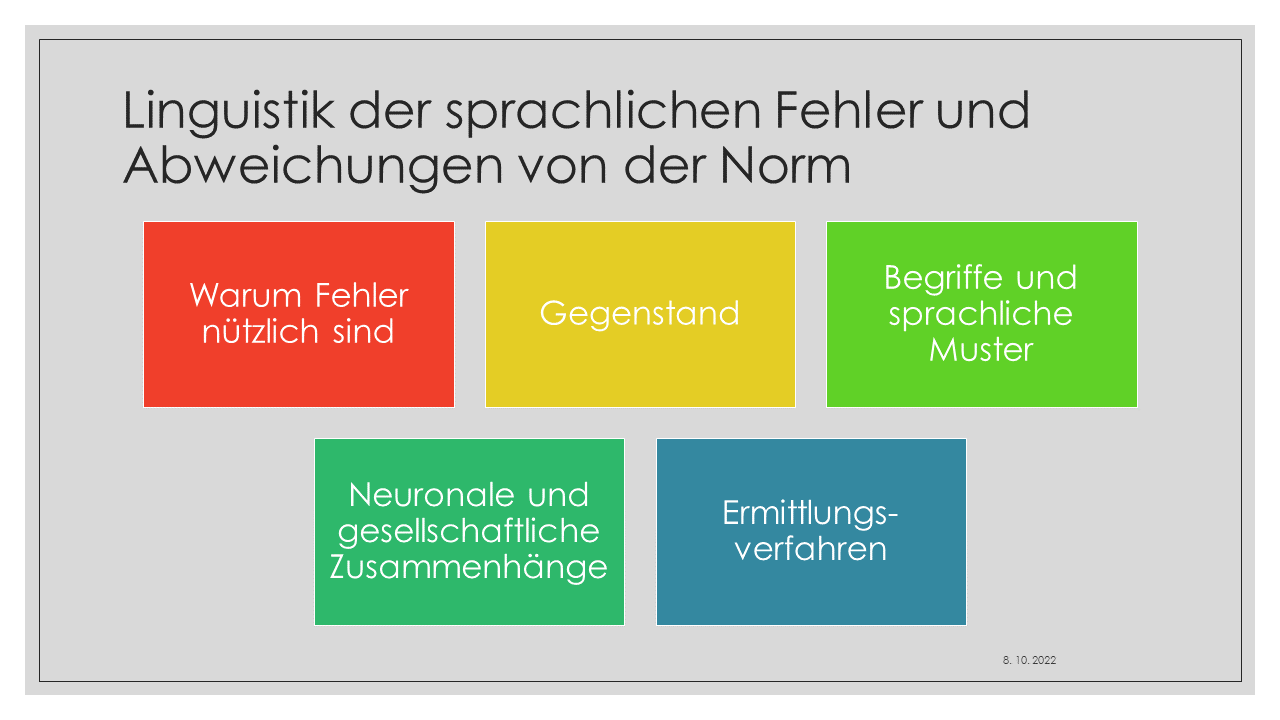
\includegraphics[width=1\textwidth,height=\textheight]{./pictures/Diapozitiv5.PNG}

Die Kernthemen der Spracherwerbsforschung lassen sich gemäß Kauschke
(2012) anhand von drei \textbf{Grundfragen} umreißen:

1. Was macht sprachliches Wissen, was macht die Beherrschung einer
Sprache aus?

2. Ist sprachliches Wissen angeboren oder wird es erlernt?

3. Wird Sprache über sprachspezifische oder über allgemein-kognitive
Mechanismen erworben?

\hypertarget{sprachbeherrschung}{%
\section{Sprachbeherrschung}\label{sprachbeherrschung}}

\textbf{Begriff des sprachlichen Wissens}

Sprache ist Bestandteil der menschlichen \textbf{Kognition}: Prozesse
der mentalen Speicherung, Aufnahme und Verarbeitung von Informationen.

Diesen Prozessen kann das \textbf{Bewusstsein} zugeschaltet sein oder
nicht.

Menge der gespeicherten Informationen (\textbf{deklaratives Wissen},
auch »Wissen, dass«)

Verfügbarkeit von informationsverarbeitenden Prozessen
(\textbf{prozedurales Wissen}, auch »Wissen, wie«).

Was macht nun sprachliches Wissen in diesem Sinne aus? Versteht man
Sprache als \textbf{gegliedertes System} von Einheiten, die durch ihre
Analysierbarkeit und ihre Kombinierbarkeit gekennzeichnet sind, so
bildet die \textbf{Entwicklung der Fähigkeit, sprachliche Einheiten zu
segmentieren und miteinander zu kombinieren, den Kern des
Spracherwerbs}.

Über den Aufbau sprachstrukturellen Wissens hinaus ist Wissen über die
\textbf{Gebrauchsbedingungen} von Sprache, ihre kommunikative Funktion
und ihren reziproken Charakter ebenfalls Gegenstand des Spracherwerbs.
Derartige anwendungsbezogene Aspekte von Sprache werden bereits
\textbf{im ersten Lebensjahr} in Austauschprozessen zwischen dem Kind
und seinen \textbf{Bezugspersonen} angebahnt und im weiteren Verlauf
ausdifferenziert.

\hypertarget{ist-sprachliches-wissen-angeboren-oder-wird-es-erlernt}{%
\section{Ist sprachliches Wissen angeboren oder wird es
erlernt?}\label{ist-sprachliches-wissen-angeboren-oder-wird-es-erlernt}}

Seit langem als Kernthema der Spracherwerbsforschung und immer wieder
neu diskutiert. Debatte um den Einfluss von Erbe und Umwelt auf die
Entwicklung von Individuen. Ausbildung dieser humanspezifischen
Fähigkeit nur möglich, wenn die sprachlernenden Menschen einer
Umgebungssprache ausgesetzt sind. Kontrovers wird diskutiert, welche
Rolle und welches Gewicht anlagebedingten Faktoren auf der einen Seite
und dem Sprachangebot der Umwelt auf der anderen Seite zukommt. Kommt
das Kind vorgeprägt für Sprache auf die Welt, ausgestattet mit
spezifischen Fähigkeiten, die in der menschlichen Entwicklungsgeschichte
entstanden sind? Entwickelt sich Sprache gemäß angeborener innerer
Voraussetzungen und vorgeprägter Reifungsprozesse entwickelt. Geht man
dagegen davon aus, dass das Kind Sprache aktiv und vorrangig durch
Kontakt und Kommunikation mit anderen Sprechern lernt.  

\hypertarget{domuxe4nenspezifik-von-sprache.}{%
\section{Domänenspezifik von
Sprache.}\label{domuxe4nenspezifik-von-sprache.}}

Wird Sprache über sprachspezifische oder allgemein-kognitive Mechanismen
erworben? Denkbar ist, dass allgemeine kognitive Prozesse auf
verschiedene Wissens- und Aufgabenbereiche anwendbar sind.

Eine andere Position besteht in der Annahme, dass für den Spracherwerb
domänenspezifisches Wissen notwendig ist, das darauf spezialisiert ist,
nur einen bestimmten Typus von Informationen zu verarbeiten.

In der Spracherwerbsforschung lassen sich drei große, traditionelle
Erklärungsparadigmen unterscheiden:

\begin{itemize}
\tightlist
\item
  Nativismus,
\item
  Interaktionismus und
\item
  Kognitivismus.
\end{itemize}

Neuere Erklärungsmodelle arbeiten auf eine Synthese hin.

\hypertarget{sec-zungenbrecher}{%
\chapter{Spracherwerbstypen}\label{sec-zungenbrecher}}

\begin{verbatim}
Error in knitr::include_graphics("pictures/kissclipart-tongue-twister-cartoon-comics-stop-consonant-82fba1d0b8543744.png"): Cannot find the file(s): "pictures/kissclipart-tongue-twister-cartoon-comics-stop-consonant-82fba1d0b8543744.png"
\end{verbatim}

\hypertarget{terminologische-unterscheidung}{%
\section{Terminologische
Unterscheidung}\label{terminologische-unterscheidung}}

In der Sprachewerbsforschung ist es möglich und üblich, verschiedene
Verben und Nomina zu verwenden, um auf verschiedene Spracherwerbstypen
Bezug zu nehmen.

\emph{Verben}: (eine Sprache) erwerben, sich (eine Sprache) aneignen,
(eine Sprache) lernen.

\emph{Nomina}: der Erwerb einer Sprache, die Aneignung einer Sprache,
das Lernen einer Sprache.

Welche semantischen Unterschiede bestehen zwischen den genannten Verben
und Nomina?

Vorschlag: Schauen Sie mal im \emph{DWDS} \url{https://www.dwds.de/}
nach und versuchen Sie festzustellen, in welchen Kontexten die Verben /
Nomina vorkommen!

Vergleichen Sie die Bedeutungen auch mit den Bedeutungen entsprechender
slowenischer und englischer Ausdrücke:

\emph{Slowenisch}: pridobiti (jezik), usvojiti (jezik), se učiti
(jezika).\\
\emph{Englisch}: acquire, learn (a language), \ldots{}

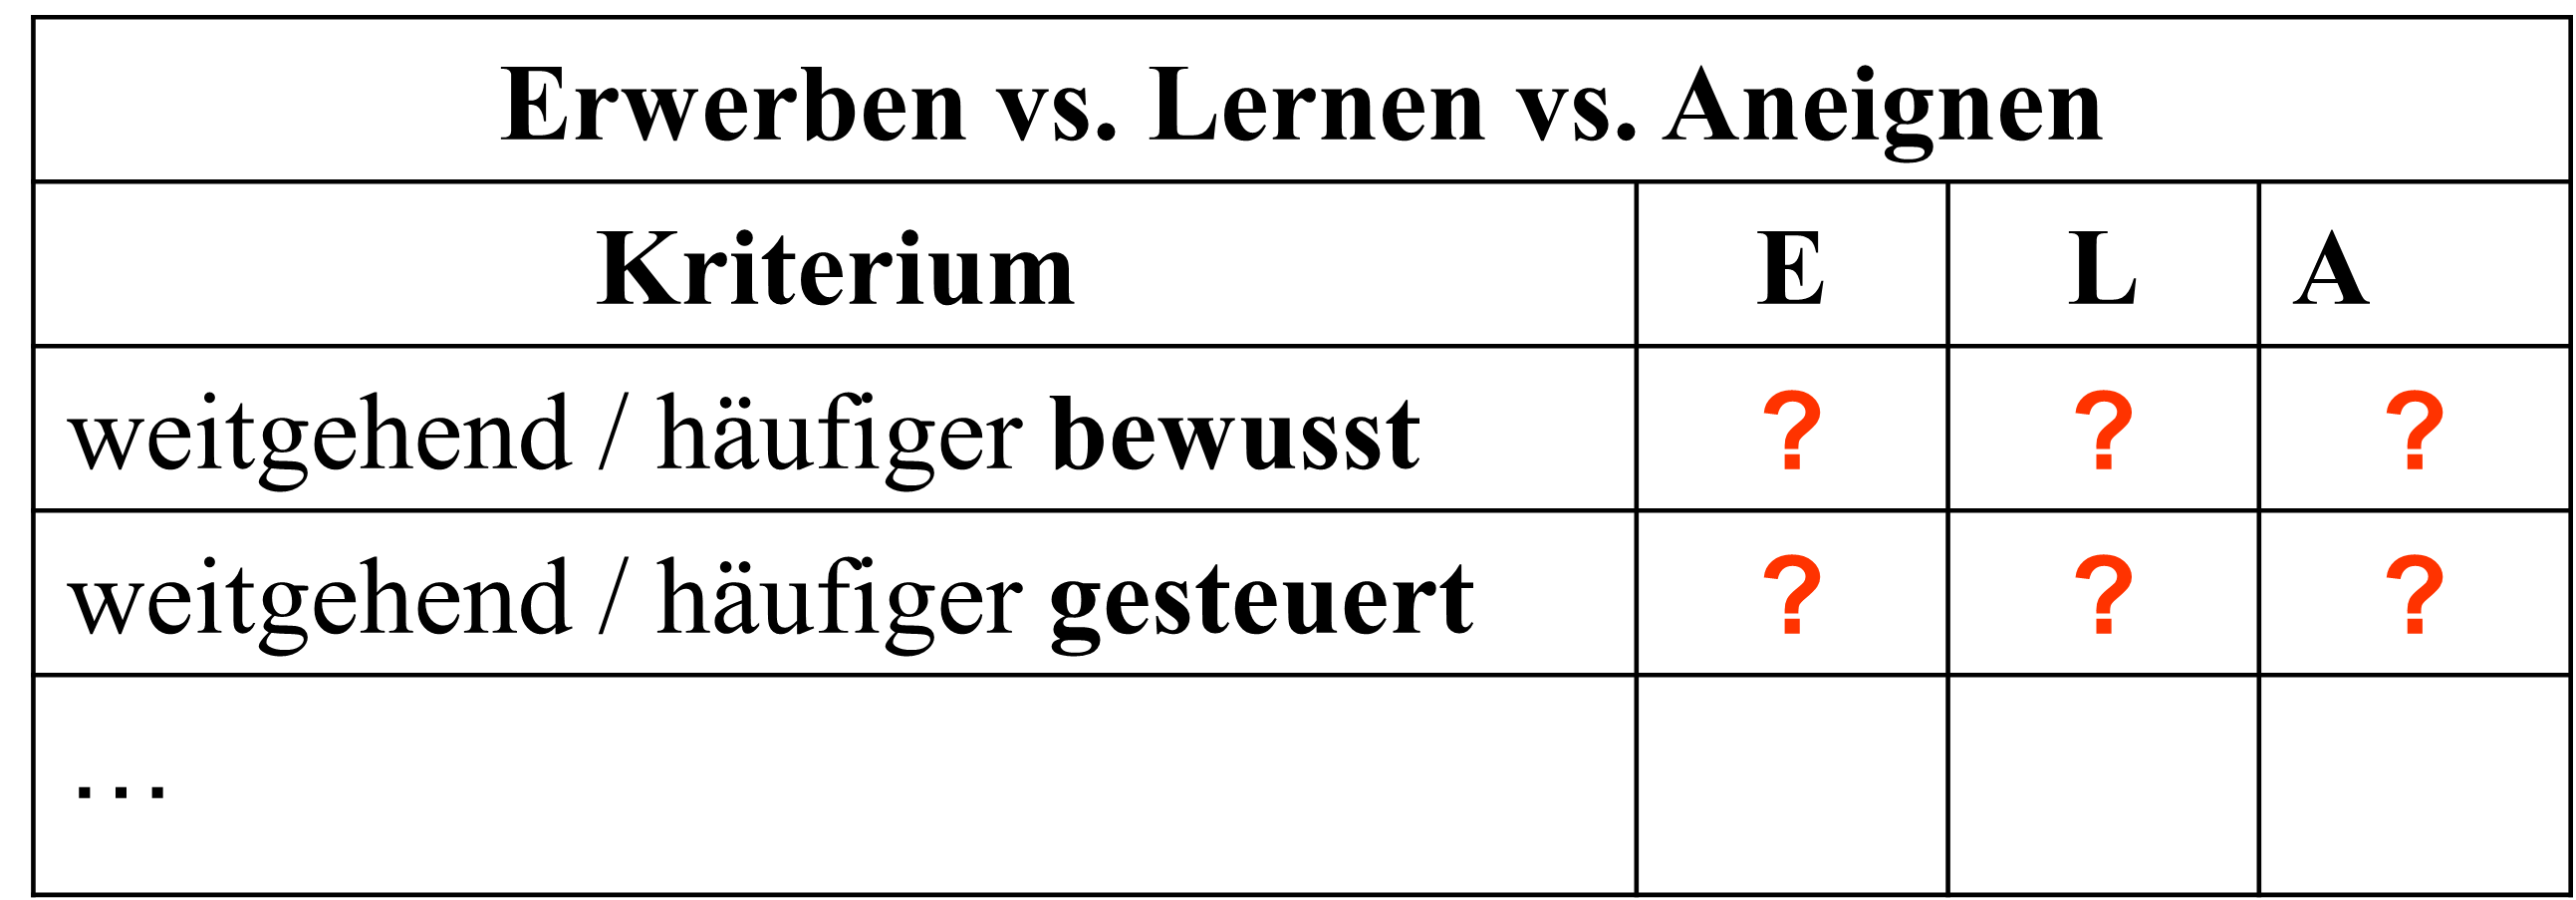
\includegraphics[width=8.62in,height=\textheight]{./pictures/termini_verben_nomen.png}

\emph{Aneignung} (A) soll als \emph{Oberbegriff} für Erwerb und Lernen
dienen. Die Aneignung einer Erstsprache ist stärker von
\emph{Erwerbsprozessen} geprägt. Die Aneignung einer Fremdsprache ist
stärker von \emph{Lernprozessen} geprägt. Die Aneignung einer
Zweitsprache (im engeren Sinne) ist je nach Fall stärker von
\emph{Erwerbs}- bzw. \emph{Lern}prozessen geprägt.

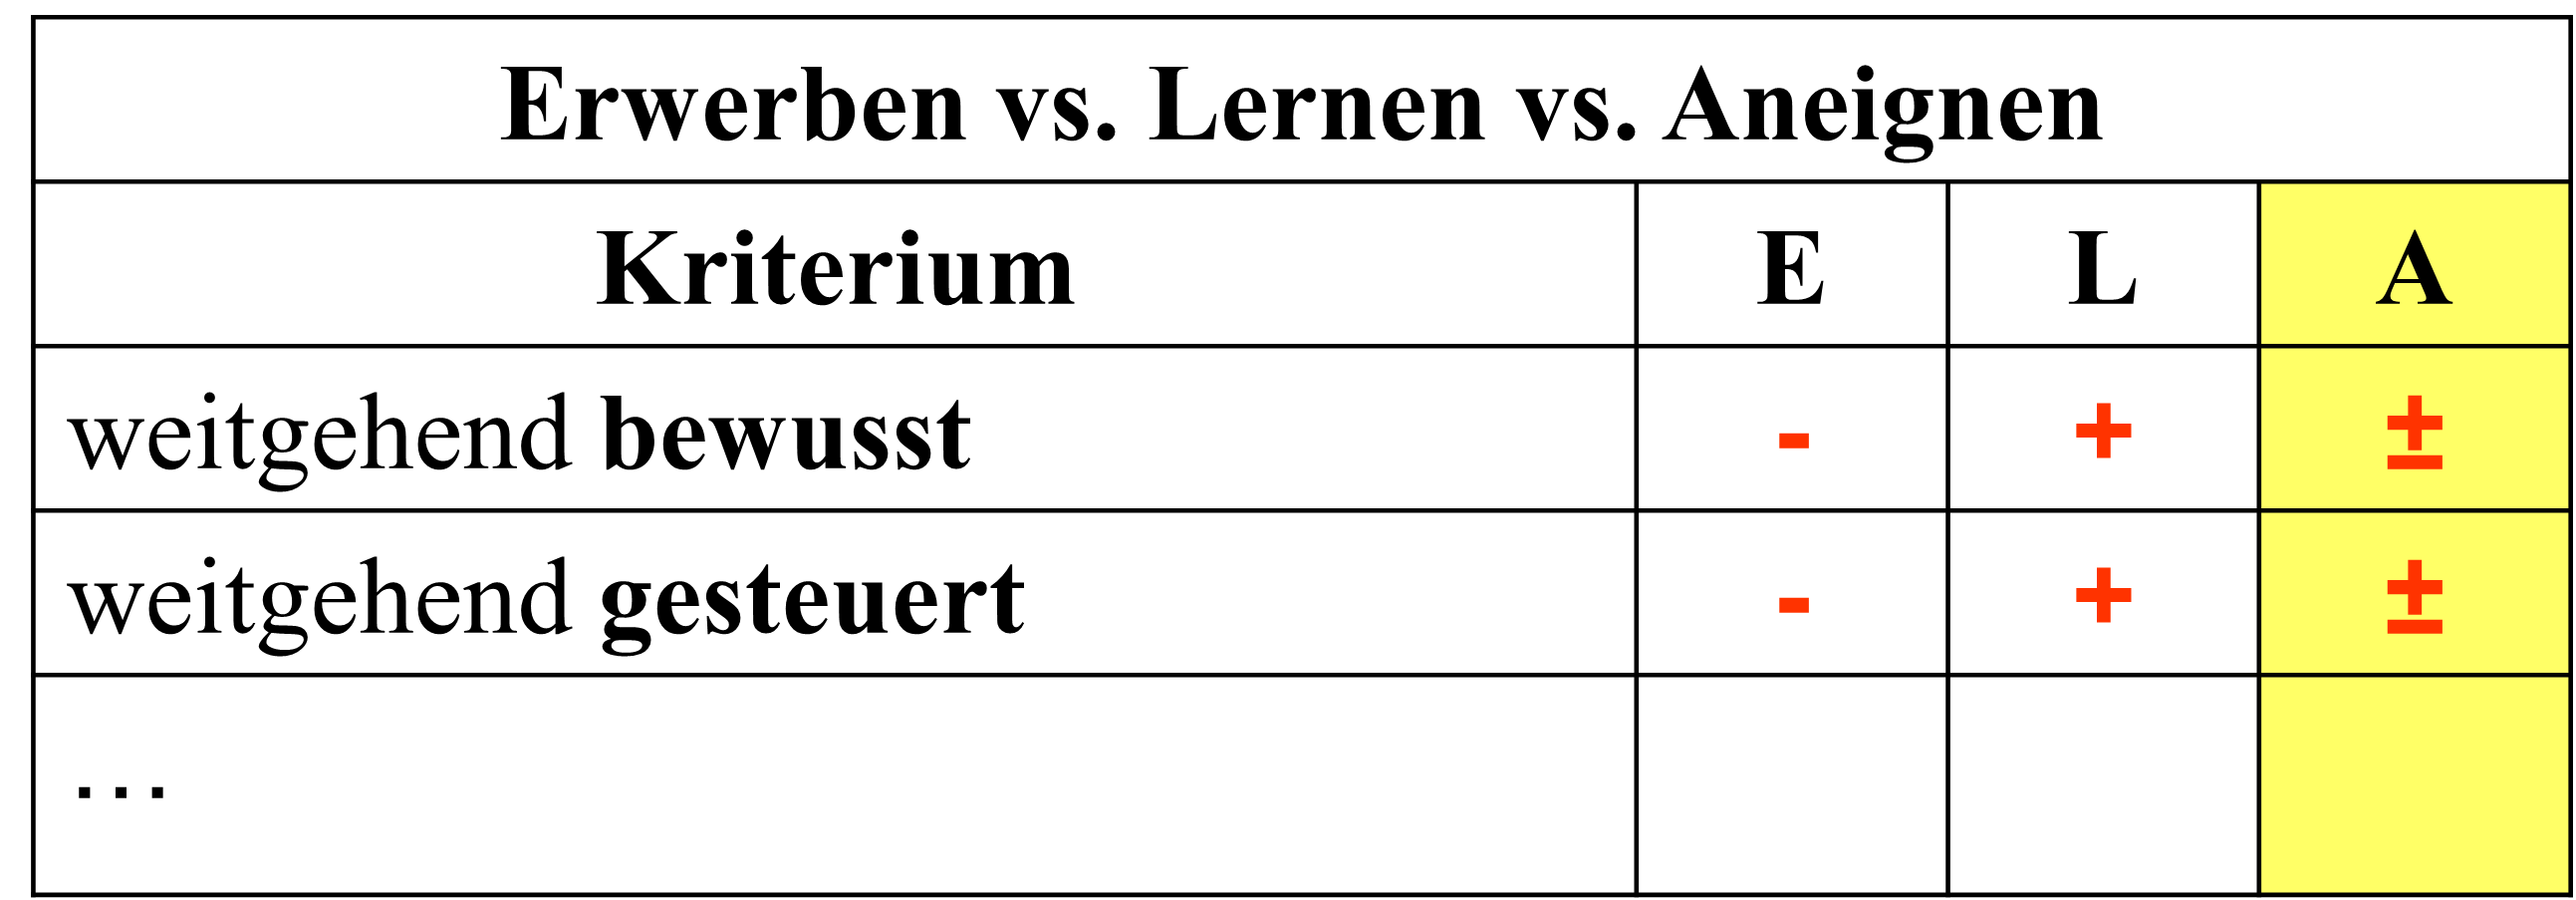
\includegraphics[width=8.62in,height=\textheight]{./pictures/termini_verben_nomen2.png}

Ihnen werden nun ein paar Videoausschnitte gezeigt, in denen die Art und
Weise beschrieben wird, wie sich Menschen eine Sprache aneignen.

Versuchen Sie, die wesentlichen Unterschiede und eventuelle
Gemeinsamkeiten herauszufinden !

\href{https://www.youtube.com/watch?v=cS_aH5wJGME}{Easy German} (Dauer:
11:07 Minuten):

\url{https://www.youtube.com/embed/cS_aH5wJGME}

\hypertarget{unterscheidungskriterien}{%
\section{Unterscheidungskriterien}\label{unterscheidungskriterien}}

Wir können eine Reihe von Kriterien verwenden, um drei
Spracherwerbstypen zu unterscheiden.

\emph{L1} steht für \emph{Erstsprache} (oft auch als
\emph{Muttersprache} bezeichnet), \emph{L2} bezieht sich auf die
\emph{Zweitsprache} und\\
\emph{FL} wird in der Tabelle für \emph{Fremdsprache} verwendet.

Der Ausdruck \emph{Muttersprache} ist bei bilingualen (d.h.
zweisprachigen) Personen nicht unbedingt zutreffend (\emph{warum?}),
darum ist \emph{Erstsprache} als Fachterminus zu bevorzugen.

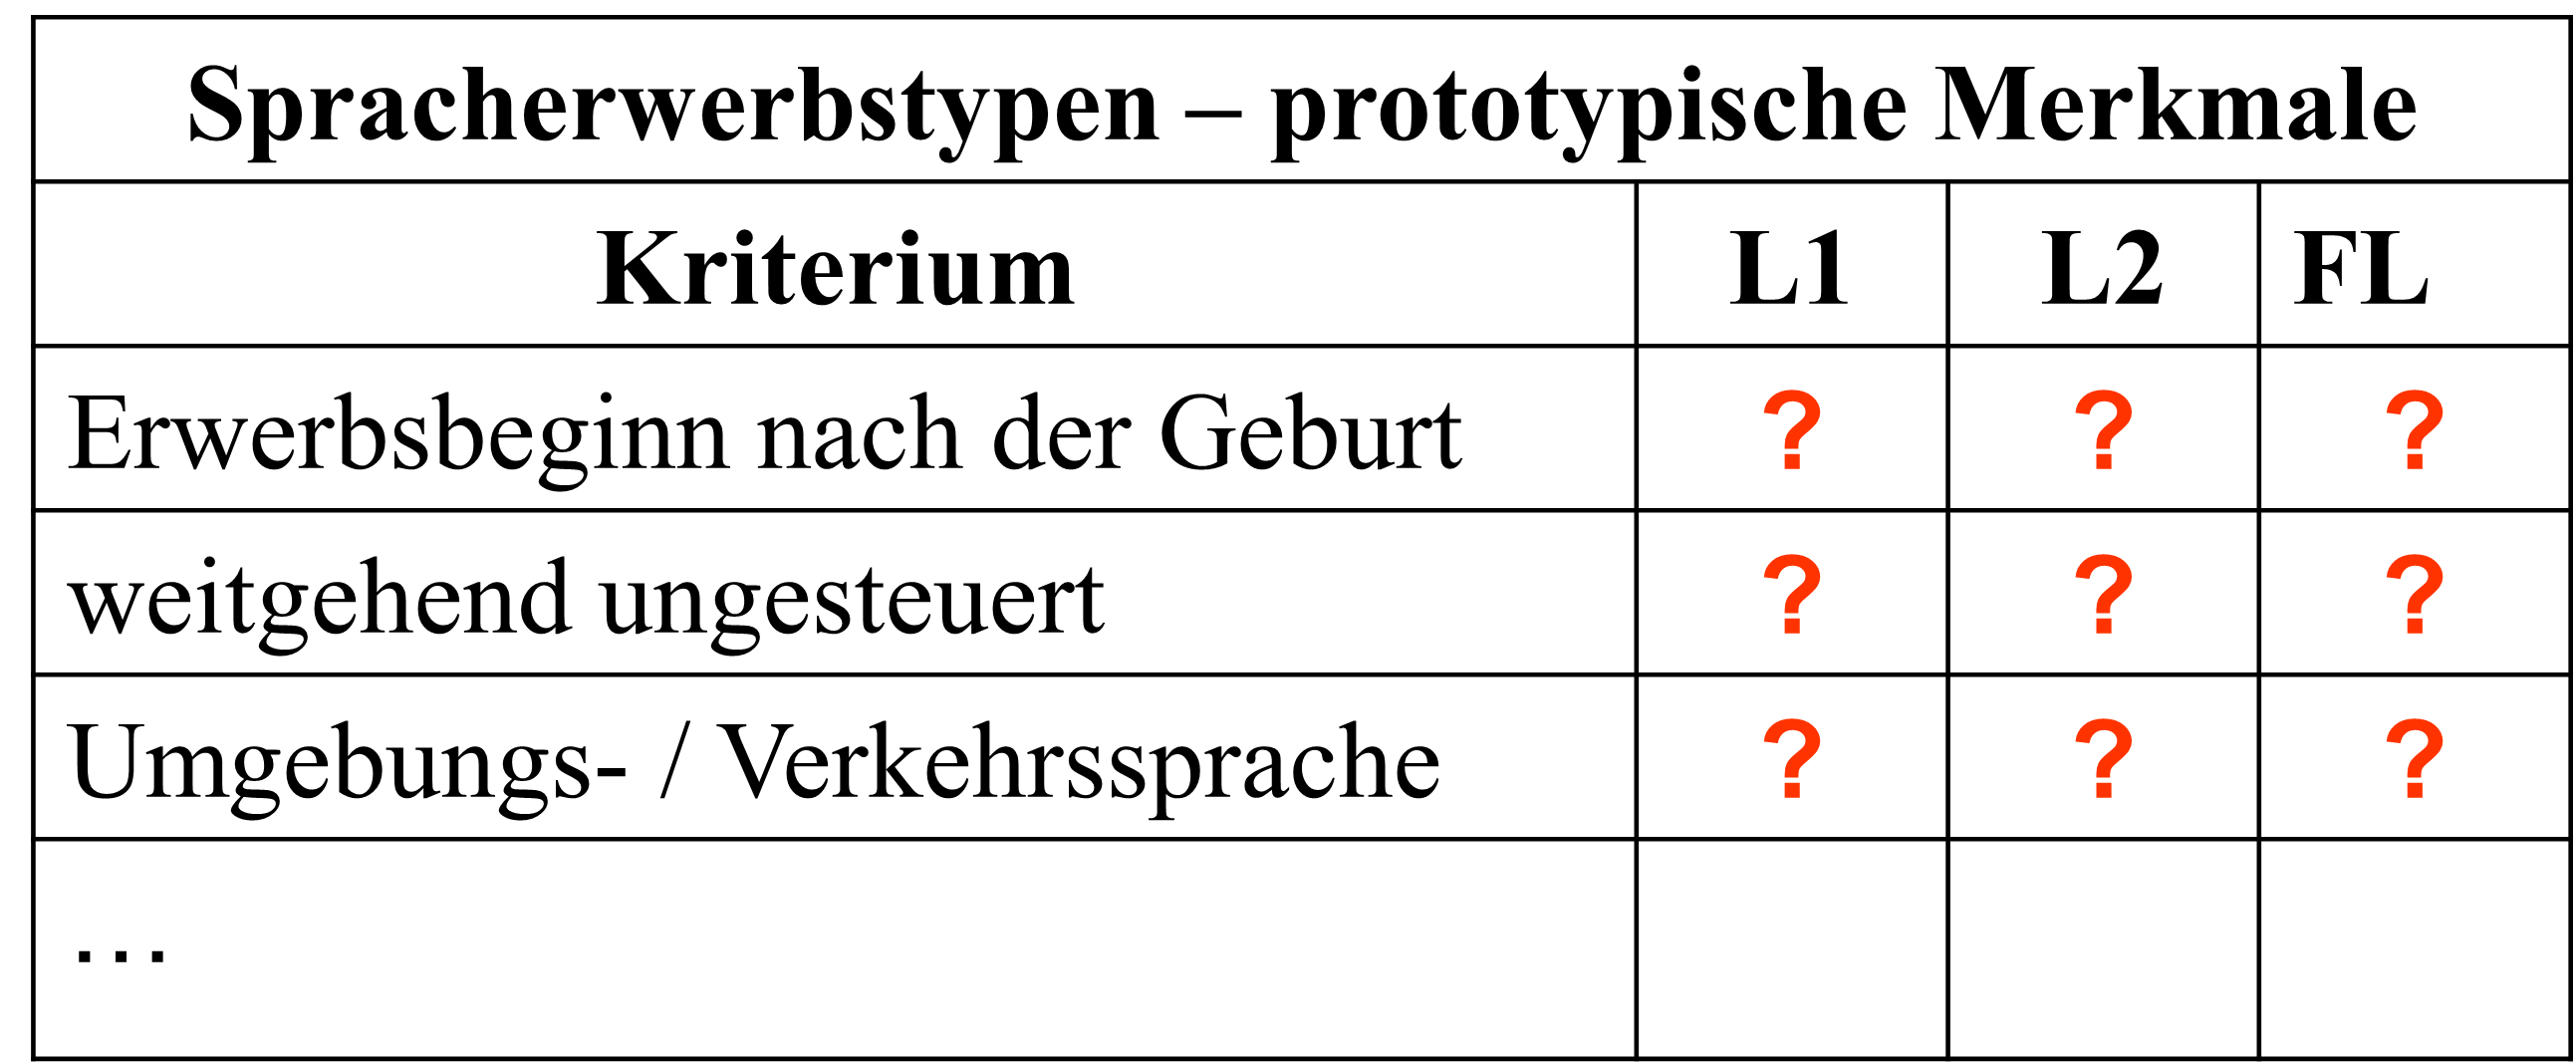
\includegraphics[width=8.62in,height=\textheight]{./pictures/spracherwerbstypen.png}

Ihnen werden nun ein paar Videoausschnitte gezeigt, in denen die Art und
Weise beschrieben wird, wie sich Menschen eine Sprache aneignen.

Versuchen Sie, die wesentlichen Unterschiede und eventuelle
Gemeinsamkeiten herauszufinden !

\href{https://www.youtube.com/watch?v=ZqObBG-NYPI}{Easy German} (Dauer:
8:46 Minuten):

\url{https://www.youtube.com/embed/ZqObBG-NYPI}

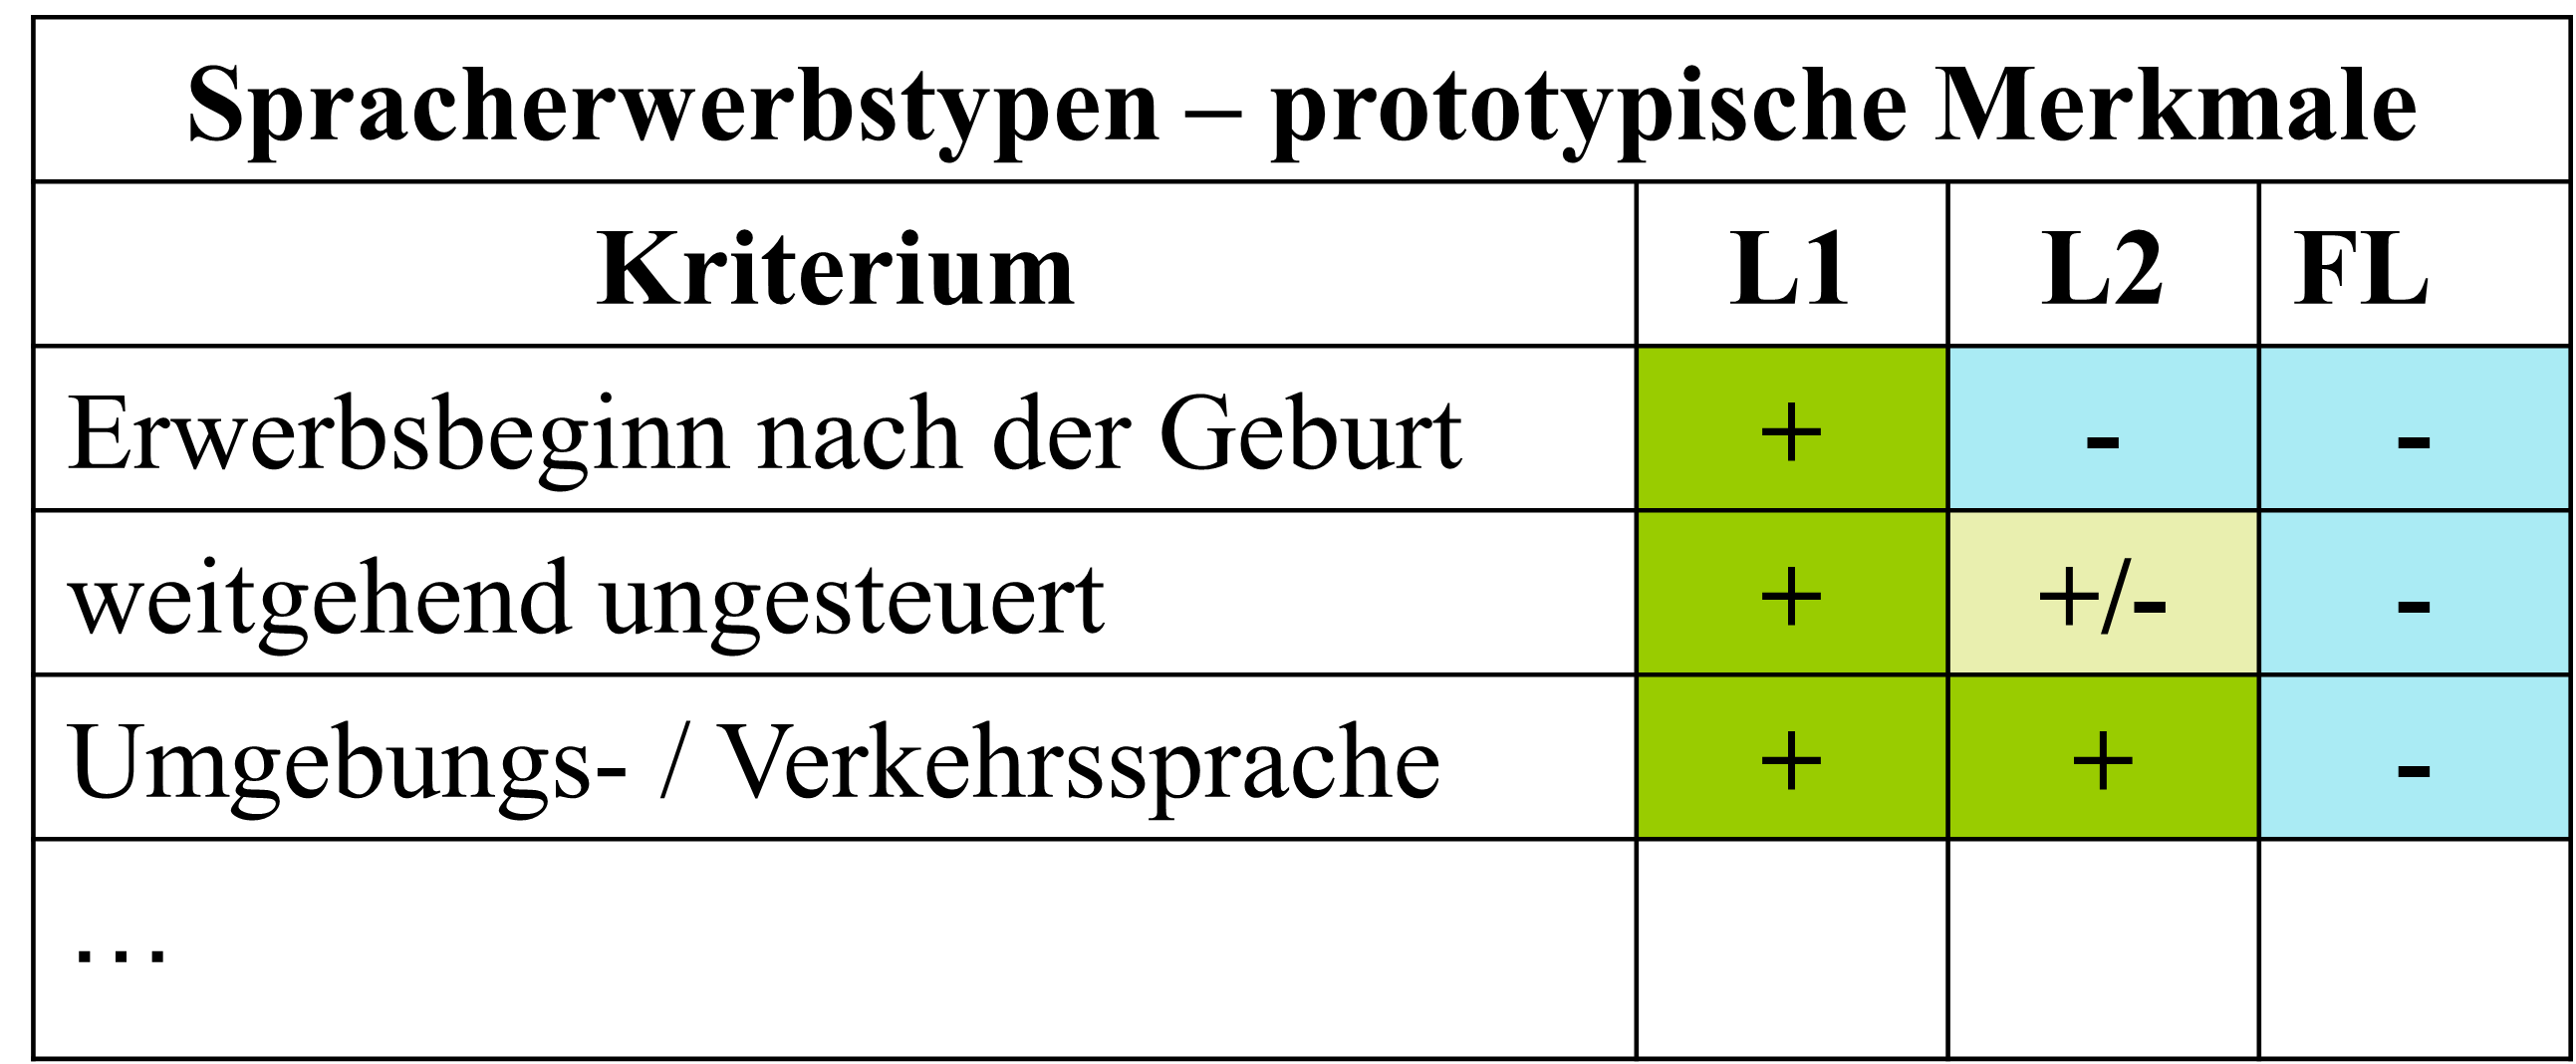
\includegraphics[width=8.62in,height=\textheight]{./pictures/spracherwerbstypen2.png}

In der Forschungsliteratur wird der Begriff \textbf{Zweitspracherwerb}

\begin{itemize}
\item
  \emph{im engeren Sinne} (wie in der zuvor gezeigten Tabelle),
\item
  bisweilen aber auch \emph{im weiteren Sinne} verwendet.
\end{itemize}

Im zweiten Fall werden Fremdspracherwerb und Zweitspracherwerb (im
engeren Sinne) als Zweitspracherwerb \textbf{zusammengefasst}. Welche
wichtige \textbf{Gemeinsamkeit} ist dafür wohl \textbf{ausschlaggebend}
?

Der Erstspracherwerb kann auch in der Form eines \textbf{doppelten
Erstspracherwerbs} (oder mehrfachen L1-Erwerbs) vorkommen.

Im Fall von bilingulaen Personen ist es auch aus neurobiologischer
Perspektive sinnvoll, zwischen \textbf{frühem} und \textbf{späten
Bilingualismus} zu unterscheiden.

\hypertarget{sec-bilingual}{%
\chapter{Vor- und Nachteile der Mehrsprachigkeit}\label{sec-bilingual}}

\begin{verbatim}
Error in knitr::include_graphics("pictures/tip-of-the-tongue1-1.png"): Cannot find the file(s): "pictures/tip-of-the-tongue1-1.png"
\end{verbatim}

Zwei- oder Mehrsprachigkeit hat nach Ansicht vieler Menschen mehrere
Vorteile. Aber viele Menschen wachsen nicht zwei- oder mehrsprachig auf.
Deshalb erhebt sich nicht nur die Frage, welche Vorteile
Mehrsprachigkeit hat, sondern auch, ob es gewisse Nachteile gibt, die
Mehrsprachigkeitsbestreben hemmen oder sogar verhindern.

Hier folgt eine Liste von Behauptungen zur Mehrsprachigkeit. Beurteilen
Sie, welche Behauptungen Sie für richtig halten und welche für nicht
haltbar.

\emph{Mobilitätsaspekte}:

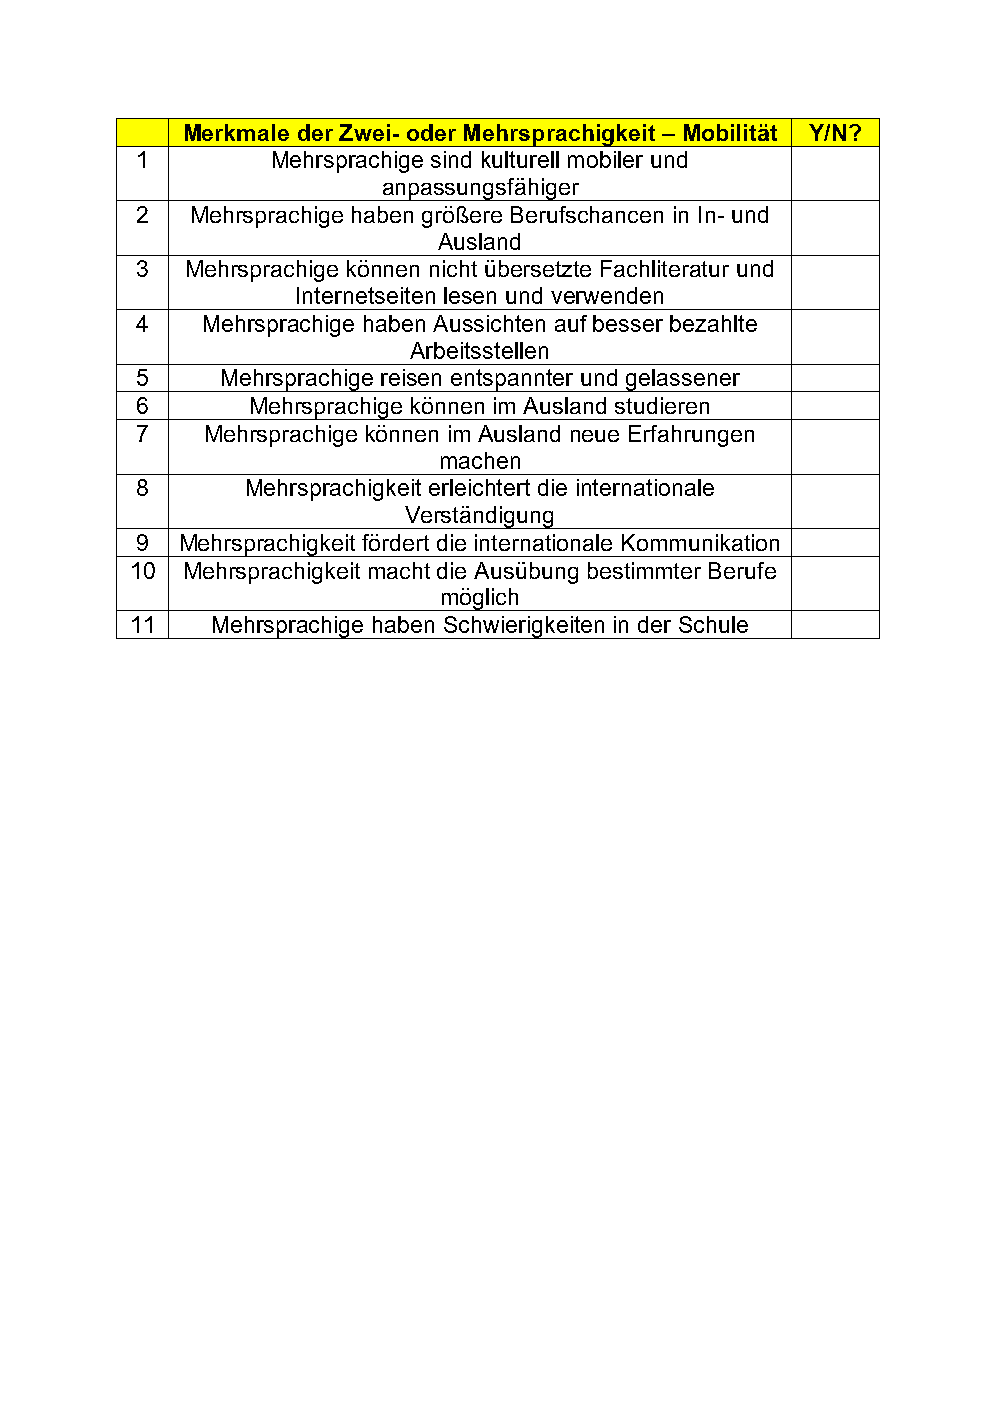
\includegraphics[width=3.31in,height=\textheight]{./pictures/Mehrsprachigkeit_Behauptungen_Page1.png}

\emph{Kulturelle Aspekte}:

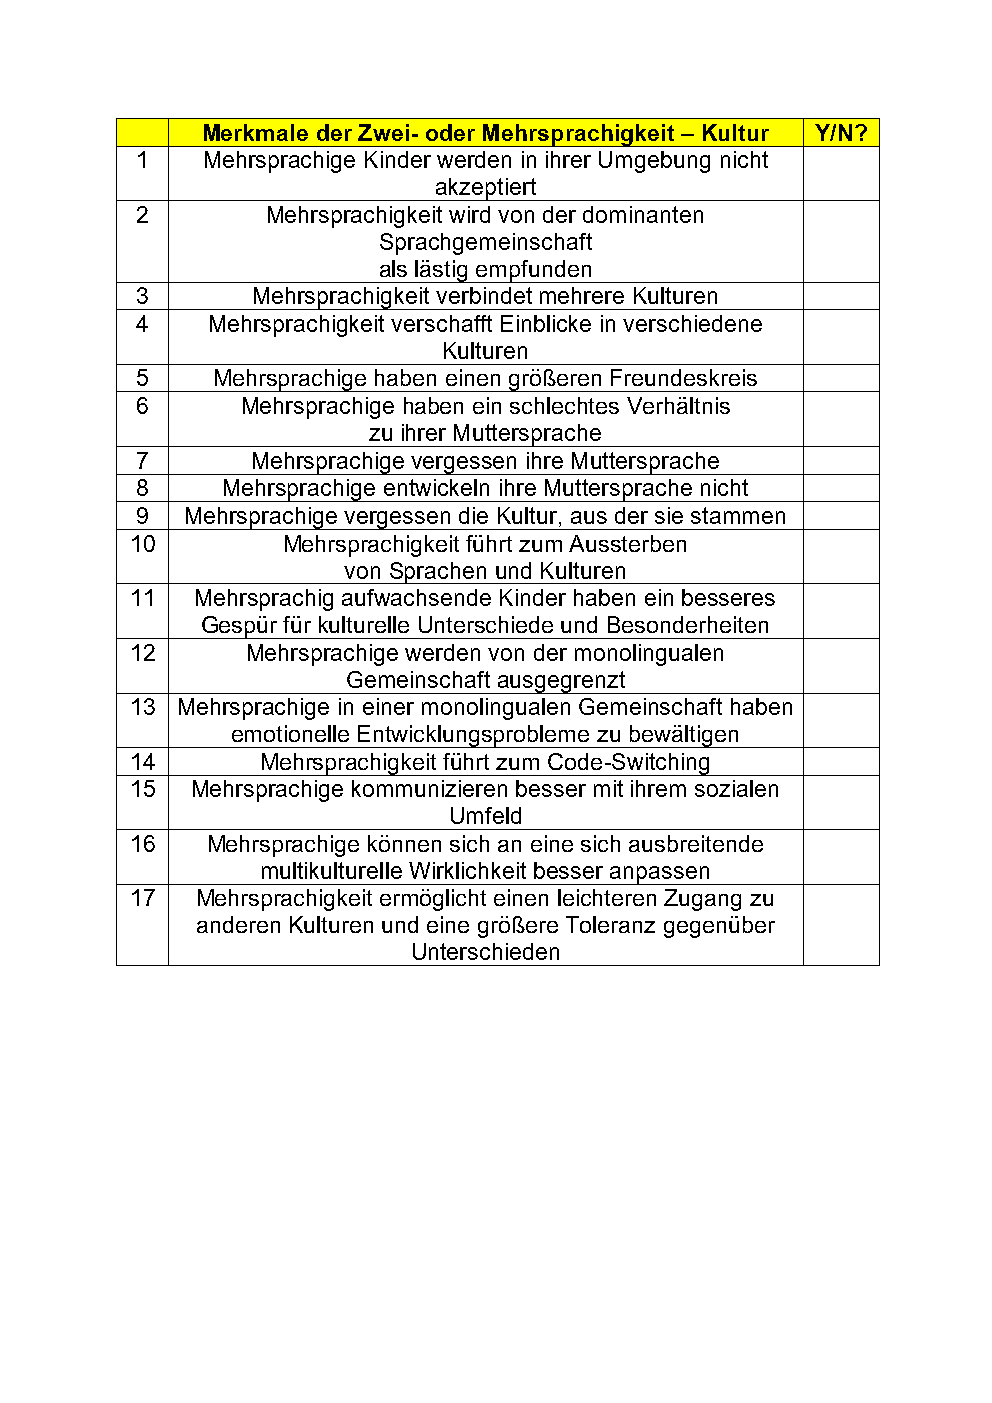
\includegraphics[width=3.31in,height=\textheight]{./pictures/Mehrsprachigkeit_Behauptungen_Page2.png}

\emph{Kognitive Aspekte}:

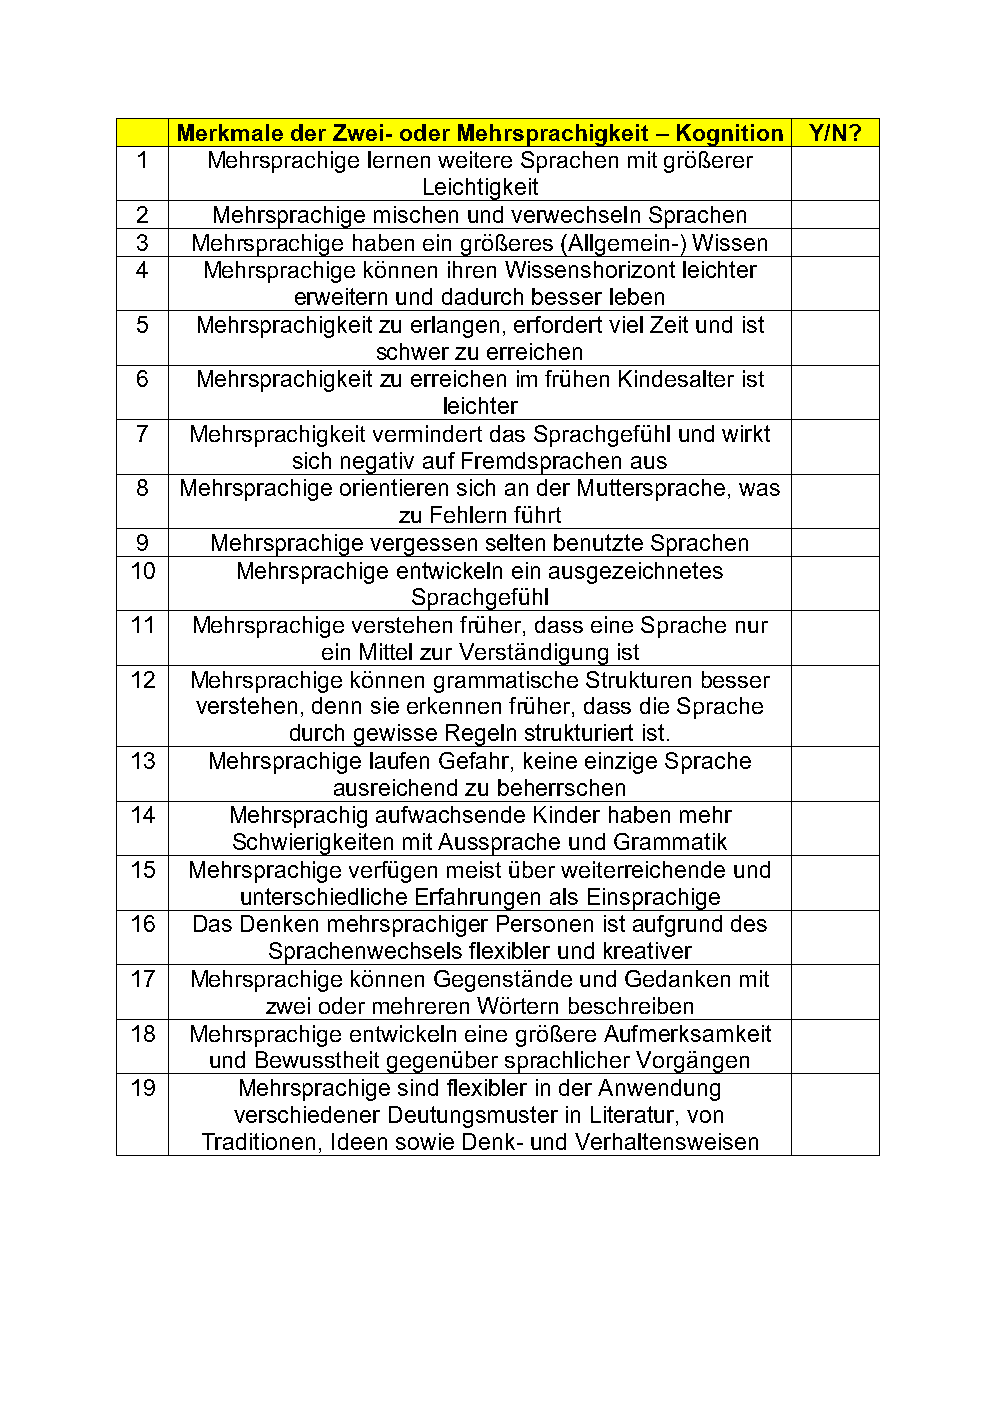
\includegraphics[width=3.31in,height=\textheight]{./pictures/Mehrsprachigkeit_Behauptungen_Page3.png}

In einem Artikel von \emph{Peter Ecke} Ecke (2008) werden \textbf{einige
Nachteile der Zwei- oder Mehrsprachigkeit} anhand von wissenschaftlichen
Studien diskutiert. Die Web-Adresse des Artikels:
\href{http://www.u.arizona.edu/~eckep/Ecke\%2008\%20Kosten\%20der\%20MS.pdf}{University
of Arizona}. Hier ist ein Abdruck der ersten Seite:

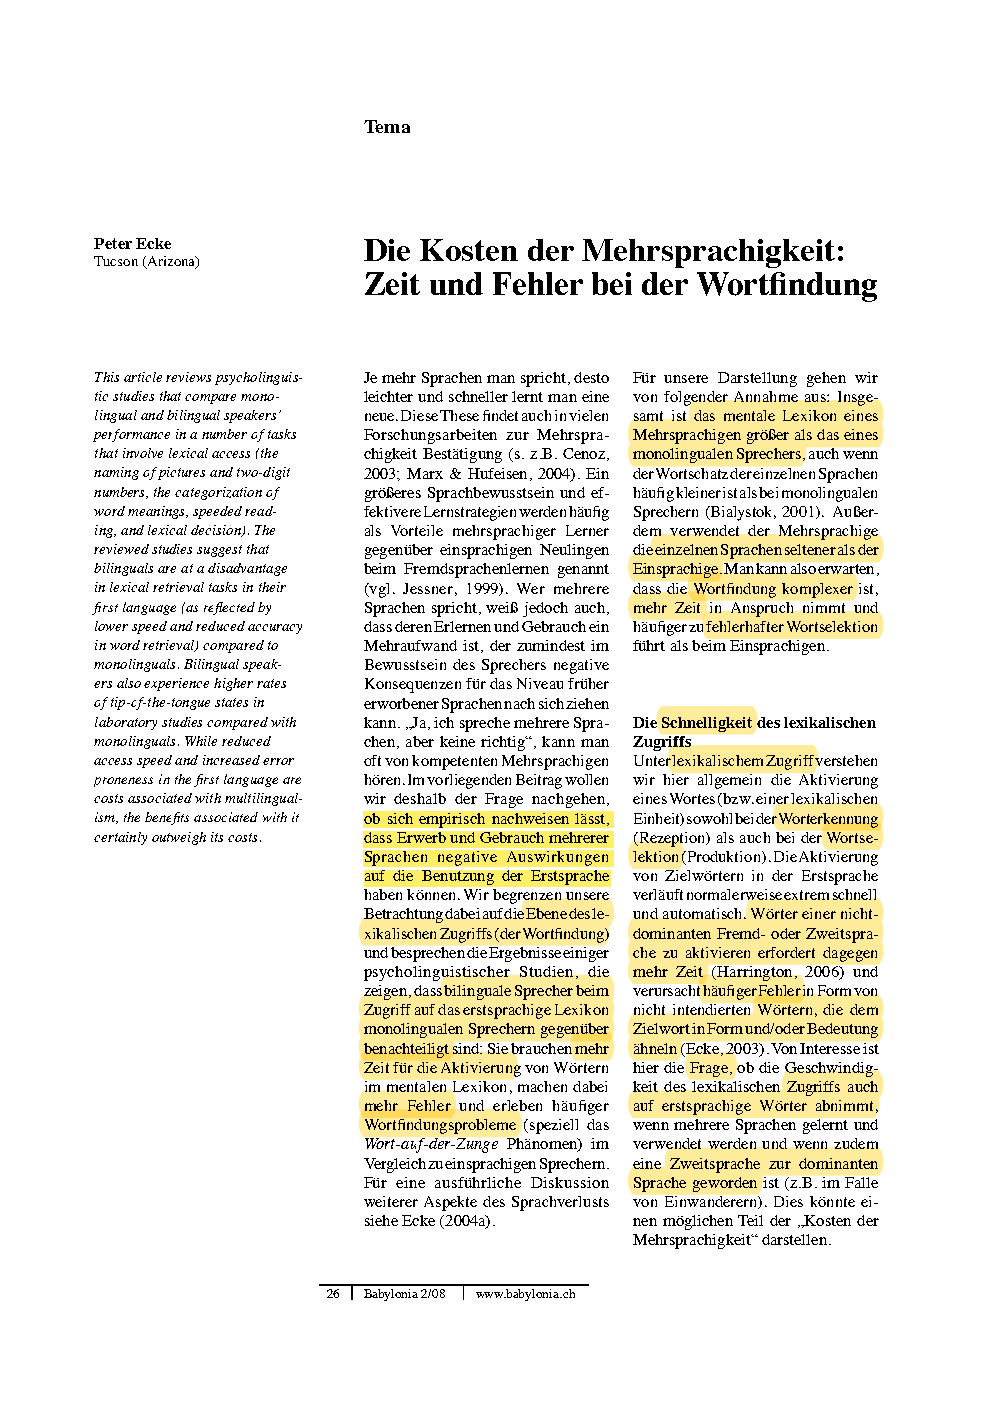
\includegraphics[width=3.31in,height=\textheight]{./pictures/TOT_bilangual_baby2_08ecke_annotated_Page1.png}

Ihnen werden nun Videos gezeigt, in denen Vorteile der
Zwei-/Mehrsprachigkeit und (vermeintliche) Nachteile erläutern werden.

Stellen Sie eine Liste der Vor- und Nachteile zusammen, damit Sie über
das Thema Mehrsprachigkeit diskutieren und entsprechend argumentieren
könen!

\href{https://www.youtube.com/watch?v=35XkRMBT28c}{Herzenssprache}
(Dauer: 7:53 Minuten):

\url{https://www.youtube.com/embed/35XkRMBT28c}

Ein weiteres Video zum Thema \emph{Mehrsprachigkeit}.

Stellen Sie eine Liste der Vor- und Nachteile zusammen, damit Sie über
das Thema Mehrsprachigkeit diskutieren und entsprechend argumentieren
könen!

\href{https://www.youtube.com/watch?v=0lJKipFitnA}{Wanderlust Monica}
(Dauer: 12:34 Minuten):

\url{https://www.youtube.com/embed/0lJKipFitnA}

Ein längeres Gespräch mit \emph{Prof.~Dr.~Jürgen Meisel} zum Thema
\emph{Mehrsprachigkeit}.

Stellen Sie eine Liste der Vor- und Nachteile zusammen, damit Sie über
das Thema Mehrsprachigkeit diskutieren und entsprechend argumentieren
könen!

\href{https://www.youtube.com/watch?v=a2Iw0jDkwYI}{Gabriel Gelman
Sprachheld} (Dauer: 43:53 Minuten):

\url{https://www.youtube.com/embed/a2Iw0jDkwYI}

Ein kürzeres Gespräch mit \emph{Prof.~Dr.~Rosemarie Tracy} über das
Thema \emph{Mehrsprachigkeit}.

Stellen Sie eine Liste der Vor- und Nachteile zusammen, damit Sie über
das Thema Mehrsprachigkeit diskutieren und entsprechend argumentieren
könen!

\href{https://www.youtube.com/watch?v=SAlTrh_76p0}{Universität Mannheim}
(Dauer: 10:51 Minuten):

\url{https://www.youtube.com/embed/SAlTrh_76p0}

Ein Vortrag von \emph{Prof.~Dr.~Rosemarie Tracy} über das Thema
\emph{Mehrsprachigkeit}.

\href{https://www.youtube.com/watch?v=vTK5-HSjbjs}{BildungsTV} (Dauer:
53:15 Minuten):

\url{https://www.youtube.com/embed/vTK5-HSjbjs}

Ein Vortrag von \emph{Prof.~Dr.~Rosemarie Tracy} über das Thema
\emph{Spracherwerb}.

\href{https://www.youtube.com/watch?v=prCbpoi-3KI}{BildungsTV} (Dauer:
1:04:48):

\url{https://www.youtube.com/embed/prCbpoi-3KI}

\hypertarget{sec-spracherwerb}{%
\chapter{Methoden in der
Spracherwerbsforschung}\label{sec-spracherwerb}}

Welche Methoden sind in der Spracherwerbsforschung anwendbar? Welche
Vor- und Nachteile haben sie im Einzelnen?

Welche Methoden werden in Kauschke (2012) beschrieben?\\
Welche Anwendungsbereiche finden sie?\\
Welche Vor- und Nachteile zeigen sich bei ihrer Anwendung?

Stellen Sie eine Präsentation zum Thema zusammen und illustrieren Sie
sie auch mit Abbildungen und Beispielen, die Sie im Internet ausfindig
gemacht haben!

\begin{figure}

{\centering 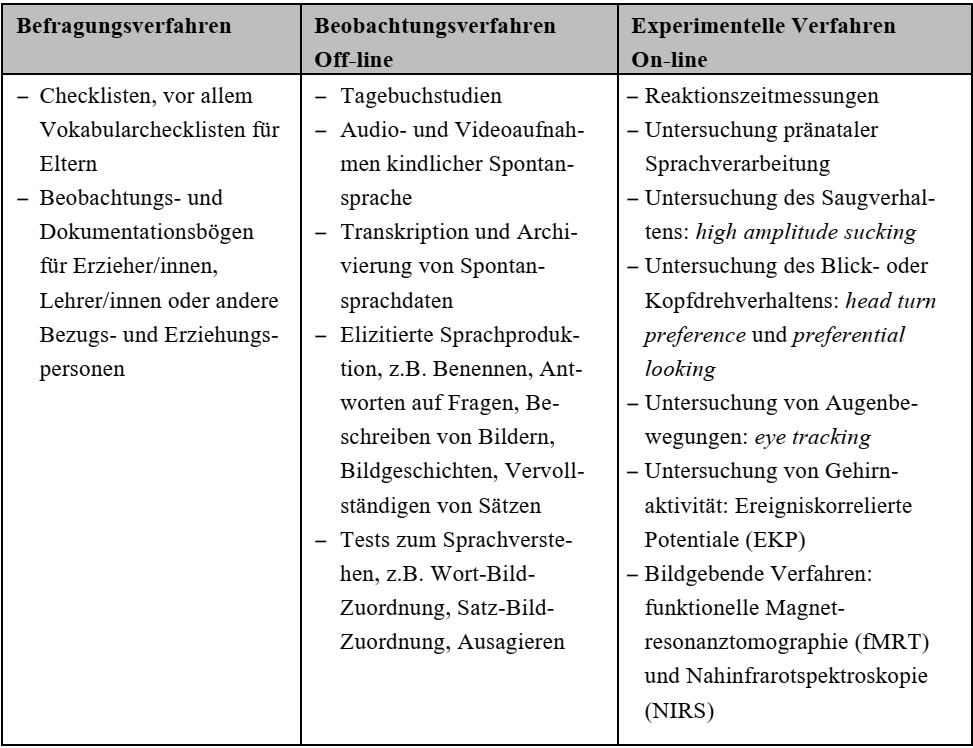
\includegraphics[width=1\textwidth,height=\textheight]{./pictures/methoden.png}

}

\caption{Übersicht über Methoden der Spracherwerbsforschung in Kauschke
(2012): 6}

\end{figure}

\hypertarget{sec-neuro}{%
\chapter{Neurobiologische und kognitive Grundlagen des
Spracherwerbs}\label{sec-neuro}}

In diesem Studienjahr haben wir uns auf folgende Themen fokussiert
(--\textgreater{} Präsentation in Teams und/oder Internetquellen):

\begin{itemize}
\item
  \textbf{Sensorisches Gedächtnis} (welche Funktion hat es?)
\item
  \textbf{Arbeitsgedächtnis} (Welche Beschränkungen hat es? Welche
  Funktion hat nach Baddelys Modell (a) die phonetische Schleife, (b)
  der visuelle Notizblock, (c) die zentrale Exekutive? Welche Rolle
  spielt Aufmerksamkeit für die Aufnahme ins Arbeitsgedächtnis? Wie kann
  man die Kapazizät des Arbeitsgedächtnisses steigern?
\item
  Wissenssysteme im \textbf{Langzeitgedächtnis} (Welche auffällige
  Unterschiede gibt es zwischen dem deklarativen und dem prozeduralen
  Langzeitgedächtnis? Welche (sprachlichen oder nicht-sprachlichen)
  Reize (Stimuli) haben größere Chancen, im Langzeitgedächtnis
  gespeichert zu werden? Welchen Einfluss haben emotional geladene Reize
  auf die Speicherung im Langzeitgedächtnis? Welche Funktion haben der
  Hippokampus, die Amygdala und frontale Hirnrindenbereiche in Bezug auf
  die langzeitige Speicherung von Einzelheiten oder Regelmäßigkeiten?)
\end{itemize}

\hypertarget{sec-theorien}{%
\chapter{Markante Thesen einflussreicher
Spracherwerbstheorien}\label{sec-theorien}}

\begin{itemize}
\item
  In welcher Hinsicht unterscheidet sich Chomskys Nativismus von
  kognivistischen und konstruktivistischen Modellen (Piaget, Tomasello)?
\item
  Welche Rolle spielt soziale Interaktion im Spracherwerb?
\item
  Worin zeigt sich, dass Nachahmungsfähigkeiten zwar wichtig sind im
  Spracherwerb, aber zur Erklärung nicht ausreichen?
\item
  Erläutern Sie die menschlichen Fähigkeiten der Mustererkennung, des
  Perspektivenwechsels und der geteilten Aufmerksamkeit im Spracherwerb!
\item
  Welchen Vorteil hat die Einordnung von Erscheinungen in Kategorien?
  Was unterscheidet Basiskategorien (z.B. Hund ) von anderen Kategorien
  (z.B. Tier, Pudel), prototypische Kategorien (z.B. Spatz) von
  nicht-prototypischen (z.B. Strauß)?
\end{itemize}

(--\textgreater{} Kauschke, Teams, \ldots)

\part{Erstspracherwerb}

\hypertarget{sec-stadien}{%
\chapter{Erstspracherwerbsstadien}\label{sec-stadien}}

\begin{verbatim}
Error in knitr::include_graphics("pictures/freudscher_versprecher_1328535.jpg"): Cannot find the file(s): "pictures/freudscher_versprecher_1328535.jpg"
\end{verbatim}

\begin{itemize}
\tightlist
\item
  Welche typischen Stadien sind im Erstspracherwerb unterscheidbar?
  (Quarks\&Co, Kauschke)
\end{itemize}

Artikelerwerb von sechs Kindern des Szagun-Korpus

\begin{itemize}
\tightlist
\item
  Beschreiben Sie den Erwerb deutscher d-Wörter, die zunächst wie
  Demonstrativpronomen auf ein außersprachliches Objekt verweisen, dann
  aber ab einem bestimmten Alter mit einem Nomen auftreten und dann die
  im Deutschen typische Artikelfunktion ausüben (d.h. Verweis auf
  bekannte oder zumindest identifizierbare Objekte in Situation und/oder
  Kontext)!
\end{itemize}

\part{Zweit- und Fremdspracherwerb}

\hypertarget{sec-gender}{%
\chapter{Entwicklungs- und transferbedingte Fehler}\label{sec-gender}}

Fehler und Abweichungen von der Zielsprache.

Kormos, Judit

\begin{itemize}
\item
  Anhand welcher Kriterien sind Transfer als Kompetenzphänomen und
  Interferenz als Performanzphänomen unterscheidbar?
\item
  Welche sprachlichen Bereiche oder Ebenen sind transferanfällig, welche
  resistenter?
\item
  Was unterscheidet entwicklungsbedingte Fehler von transferbedingten
  Fehlern?
\item
  Erläutern Sie, warum die Kontrastivhypothese nicht ausreichte, um
  bestimmte Fehler im Zweit- und Fremdspracherwerb zu erklären und dies
  zu neuen theoretischen Ansätzen führt (z.B. Identitätshypothese,
  Interlanguage-Hypothese)? ( s. Teams Zweitspracherwerb: L1 als Hilfe
  oder Hindernis, Hochländer: Fehlerkunde, Kupisch, Cantone \ldots{} in
  meiner Präsentation, Hypothesen von Krashen)
\item
  Beschreiben Sie sprachliche Fehler, die Sie entweder auf einen
  Einfluss der Erstsprache (Transfer oder Interferenz) oder als
  entwicklungsbedingte Fehler (die sich nicht auf die L1 zurückführen
  lassen) einordnen können!
\item
  Verwenden Sie zu diesem Zweck die Aufsätze der Mittelschüler, die wir
  schon während des Unterrichts analysiert haben, oder die Aufsätze der
  Studierenden (Teams: Zweitspracherwerb)!
\end{itemize}

\bookmarksetup{startatroot}

\hypertarget{abschlieuxdfende-bemerkungen}{%
\chapter{Abschließende Bemerkungen}\label{abschlieuxdfende-bemerkungen}}

Einige Hinweise für \emph{\texttt{selbständige}} Textanalysen. 🤗

\{\{ \textless{} include \_WM\_Presentation.qmd \textgreater{} \}\}

\hypertarget{fontawesome}{%
\section{Fontawesome}\label{fontawesome}}

In the terminal use:\\
quarto install quarto-ext/fontawesome

This extension folder has to be installed in every project.

After installation, use curly braces to include fa icons / or use html
code (e.g.~copy free icons from https://fontawesome.com , namely:
https://fontawesome.com/start).

\faIcon{envelope} - the code for an envelope

\faIcon{facebook} - the code for brands like facebook

For icon-styling go to https://github.com/quarto-ext/fontawesome:

\faIcon{windows}

On https://fontawesome.com/docs, there is information on how to change
the color of the icons, e.g.~in the Styling section, Basics.

{ }

Rotated icons:

Possible to include animated icons:

\hypertarget{callout-types}{%
\section{Callout Types}\label{callout-types}}

\begin{tcolorbox}[enhanced jigsaw, bottomrule=.15mm, left=2mm, opacityback=0, leftrule=.75mm, toptitle=1mm, titlerule=0mm, colback=white, breakable, colbacktitle=quarto-callout-note-color!10!white, colframe=quarto-callout-note-color-frame, bottomtitle=1mm, opacitybacktitle=0.6, coltitle=black, title=\textcolor{quarto-callout-note-color}{\faInfo}\hspace{0.5em}{Note}, arc=.35mm, rightrule=.15mm, toprule=.15mm]

Note that there are five types of callouts, including: \texttt{note},
\texttt{warning}, \texttt{important}, \texttt{tip}, and
\texttt{caution}.

\end{tcolorbox}

\begin{tcolorbox}[enhanced jigsaw, bottomrule=.15mm, left=2mm, opacityback=0, leftrule=.75mm, toptitle=1mm, titlerule=0mm, colback=white, breakable, colbacktitle=quarto-callout-tip-color!10!white, colframe=quarto-callout-tip-color-frame, bottomtitle=1mm, opacitybacktitle=0.6, coltitle=black, title=\textcolor{quarto-callout-tip-color}{\faLightbulb}\hspace{0.5em}{Tip With Caption / Tipp mit Titel}, arc=.35mm, rightrule=.15mm, toprule=.15mm]

This is an example of a callout with a caption.

\end{tcolorbox}

\begin{tcolorbox}[enhanced jigsaw, bottomrule=.15mm, left=2mm, opacityback=0, leftrule=.75mm, toptitle=1mm, titlerule=0mm, colback=white, breakable, colbacktitle=quarto-callout-important-color!10!white, colframe=quarto-callout-important-color-frame, bottomtitle=1mm, opacitybacktitle=0.6, coltitle=black, title=\textcolor{quarto-callout-important-color}{\faExclamation}\hspace{0.5em}{Important}, arc=.35mm, rightrule=.15mm, toprule=.15mm]

Das ist wichtig.

\end{tcolorbox}

\begin{tcolorbox}[enhanced jigsaw, bottomrule=.15mm, left=2mm, opacityback=0, leftrule=.75mm, toptitle=1mm, titlerule=0mm, colback=white, breakable, colbacktitle=quarto-callout-warning-color!10!white, colframe=quarto-callout-warning-color-frame, bottomtitle=1mm, opacitybacktitle=0.6, coltitle=black, title=\textcolor{quarto-callout-warning-color}{\faExclamationTriangle}\hspace{0.5em}{Warning}, arc=.35mm, rightrule=.15mm, toprule=.15mm]

Warning

\end{tcolorbox}

\begin{tcolorbox}[enhanced jigsaw, bottomrule=.15mm, left=2mm, opacityback=0, leftrule=.75mm, toptitle=1mm, titlerule=0mm, colback=white, breakable, colbacktitle=quarto-callout-caution-color!10!white, colframe=quarto-callout-caution-color-frame, bottomtitle=1mm, opacitybacktitle=0.6, coltitle=black, title=\textcolor{quarto-callout-caution-color}{\faFire}\hspace{0.5em}{Expand To Learn About Collapse}, arc=.35mm, rightrule=.15mm, toprule=.15mm]

This is an example of a `folded' caution callout that can be expanded by
the user. You can use \texttt{collapse="true"} to collapse it by default
or \texttt{collapse="false"} to make a collapsible callout that is
expanded by default.

\end{tcolorbox}

\hypertarget{diagrammer-mermaid}{%
\section{DiagrammeR mermaid}\label{diagrammer-mermaid}}

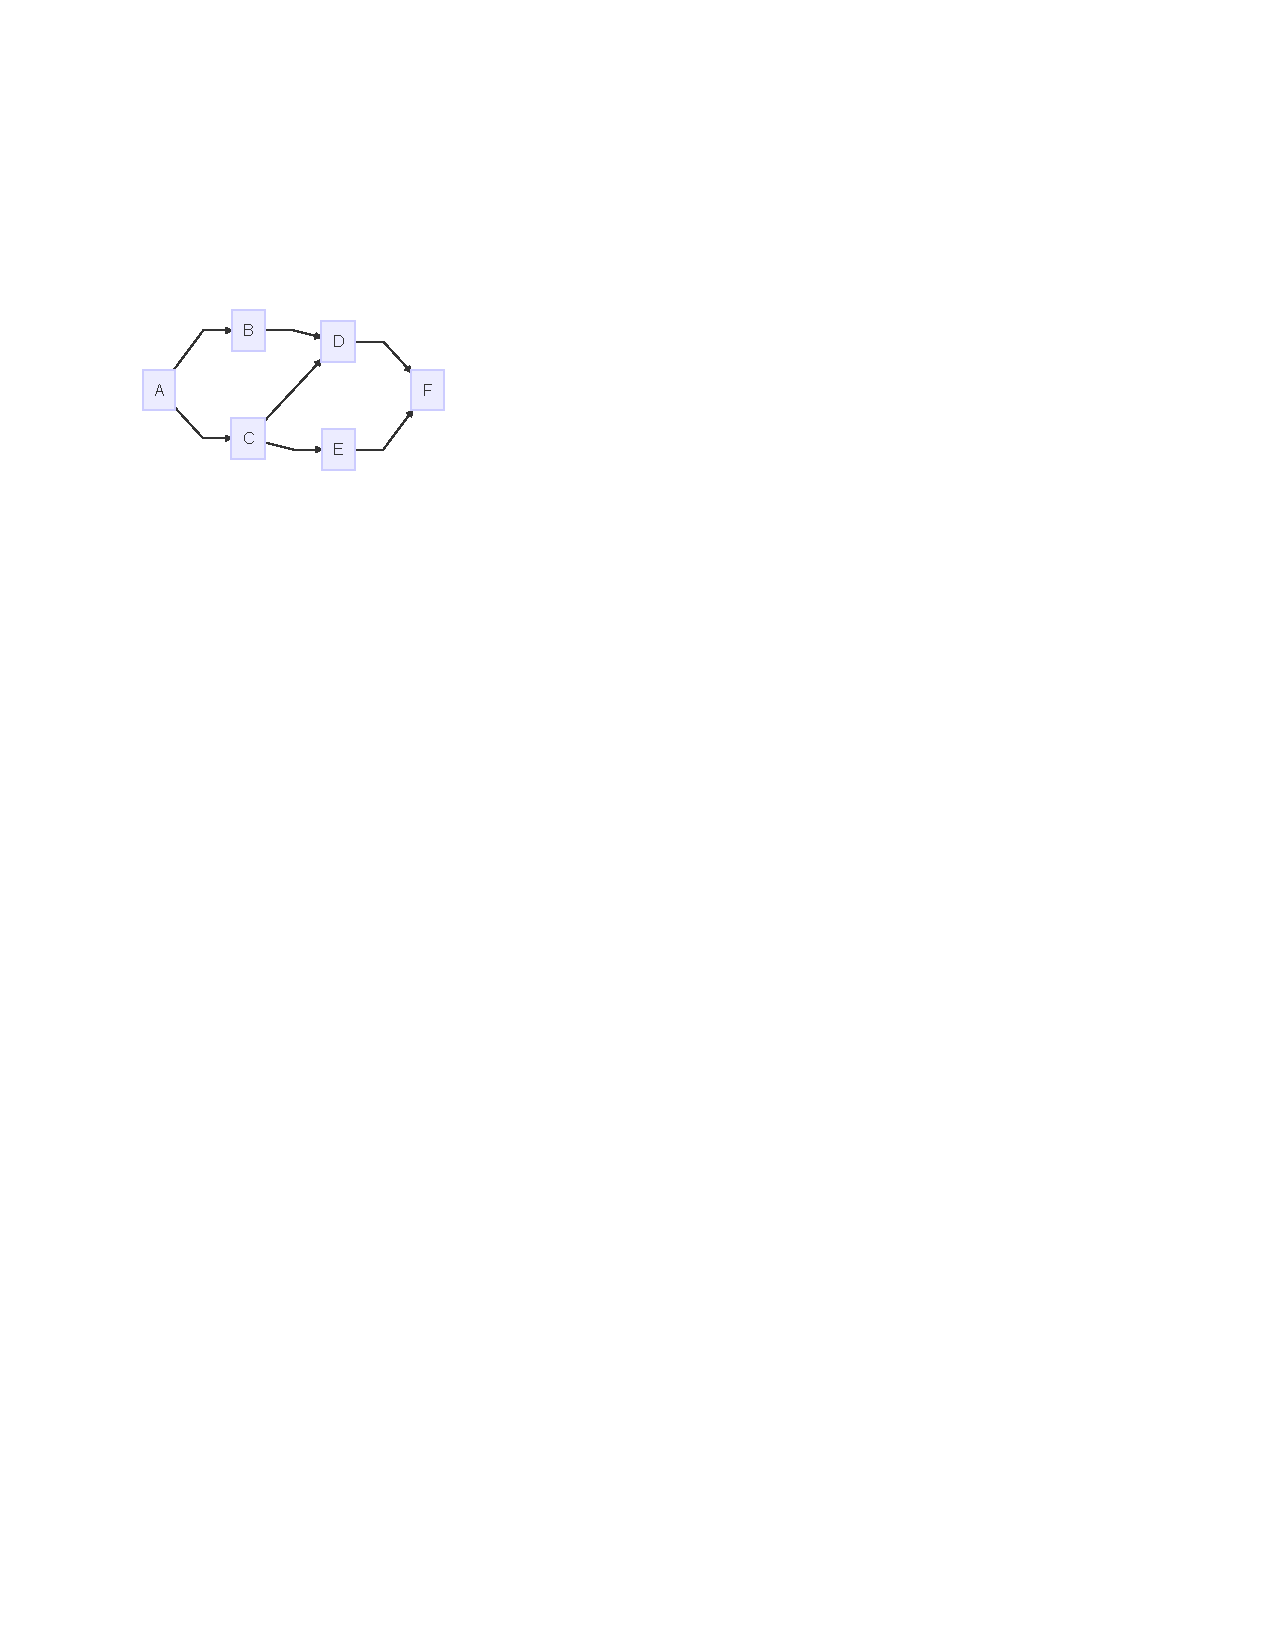
\includegraphics{./summary_files/figure-pdf/unnamed-chunk-1-1.pdf}

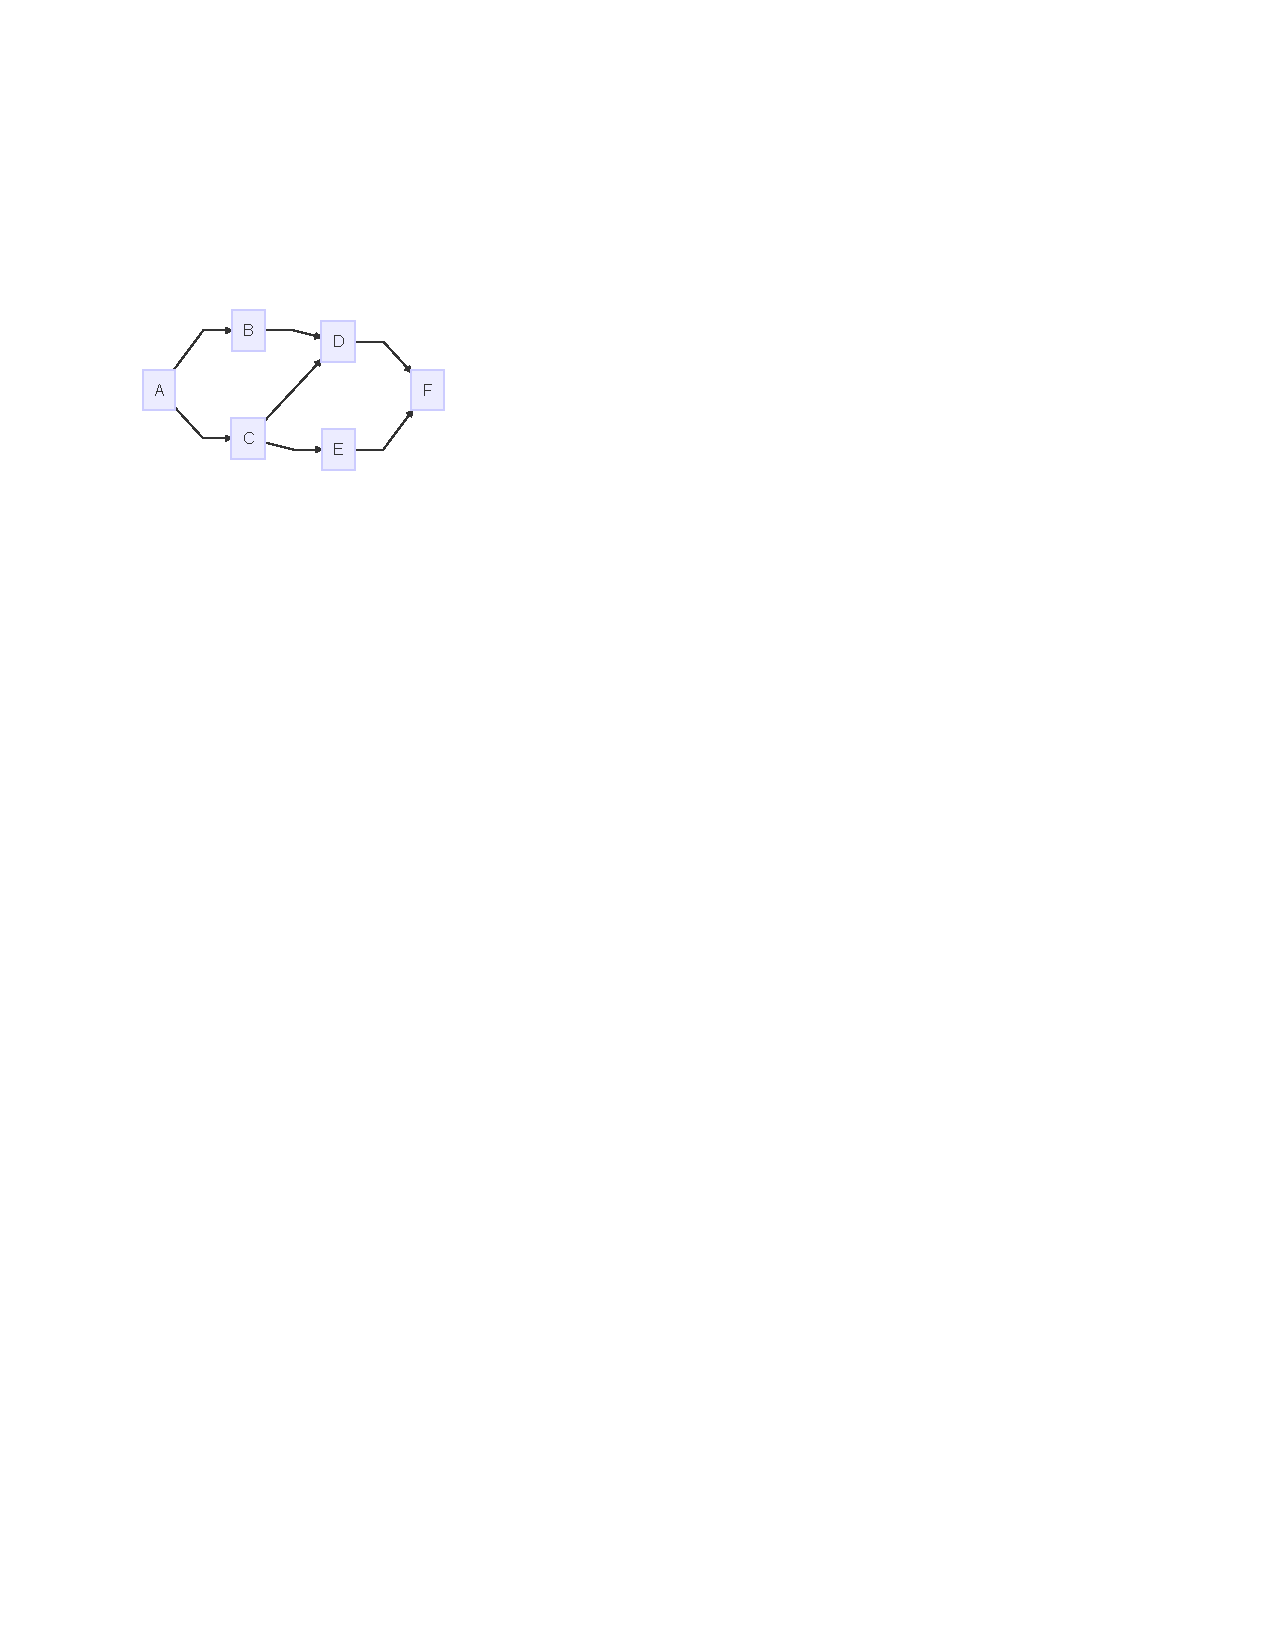
\includegraphics{./summary_files/figure-pdf/unnamed-chunk-2-1.pdf}

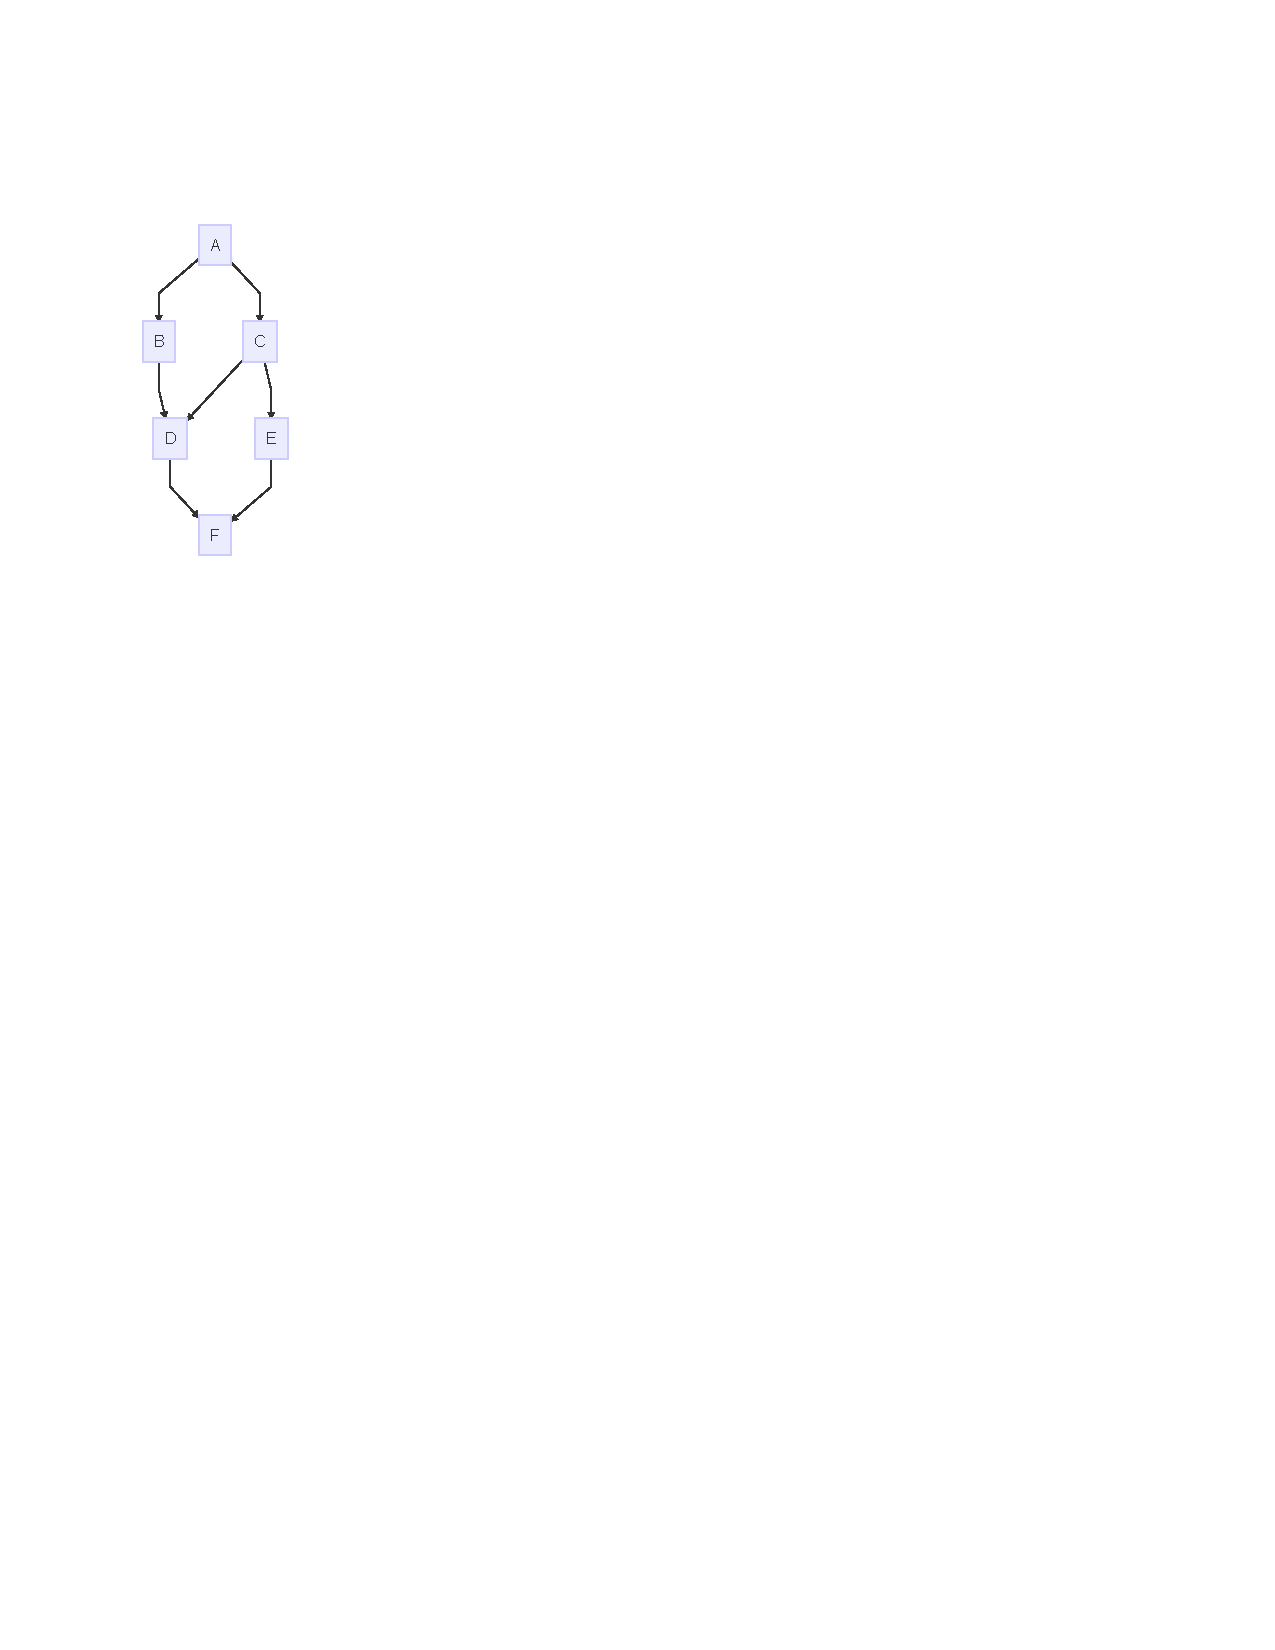
\includegraphics{./summary_files/figure-pdf/unnamed-chunk-3-1.pdf}

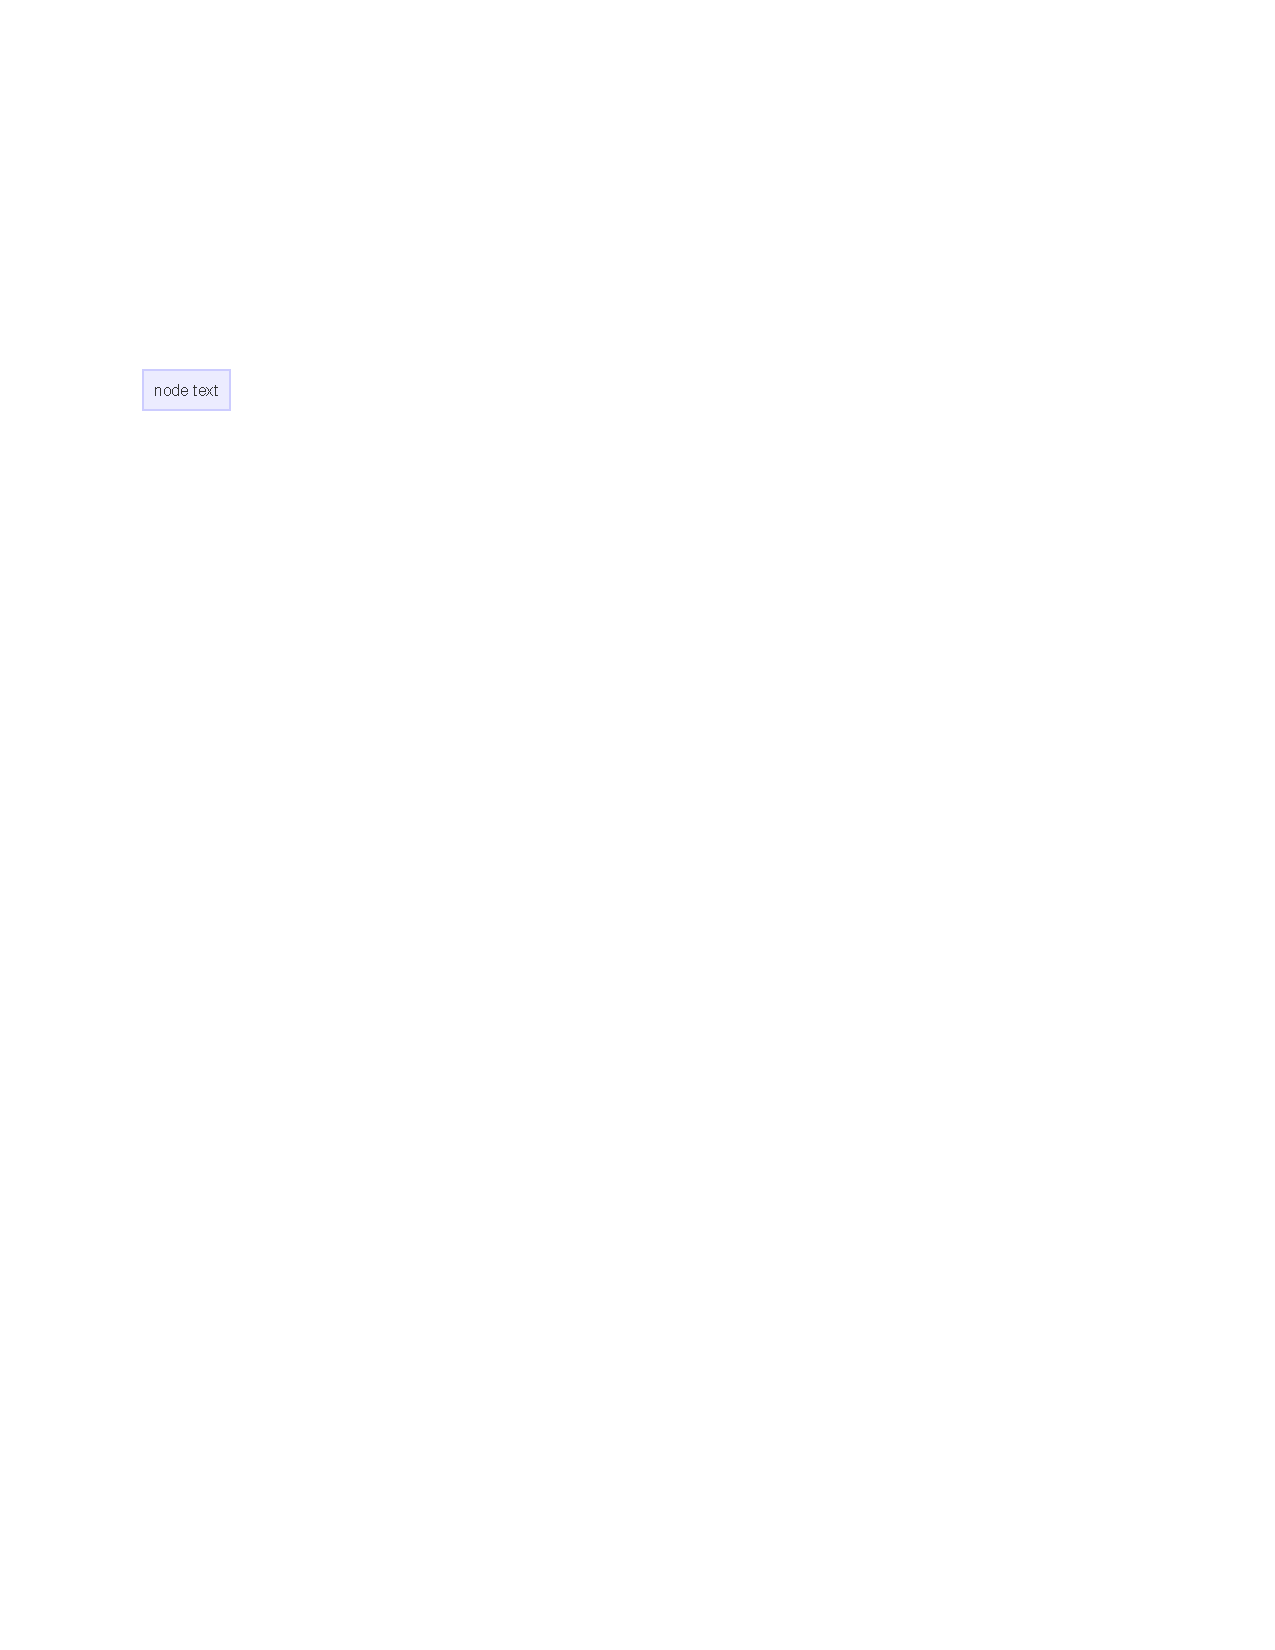
\includegraphics{./summary_files/figure-pdf/unnamed-chunk-4-1.pdf}

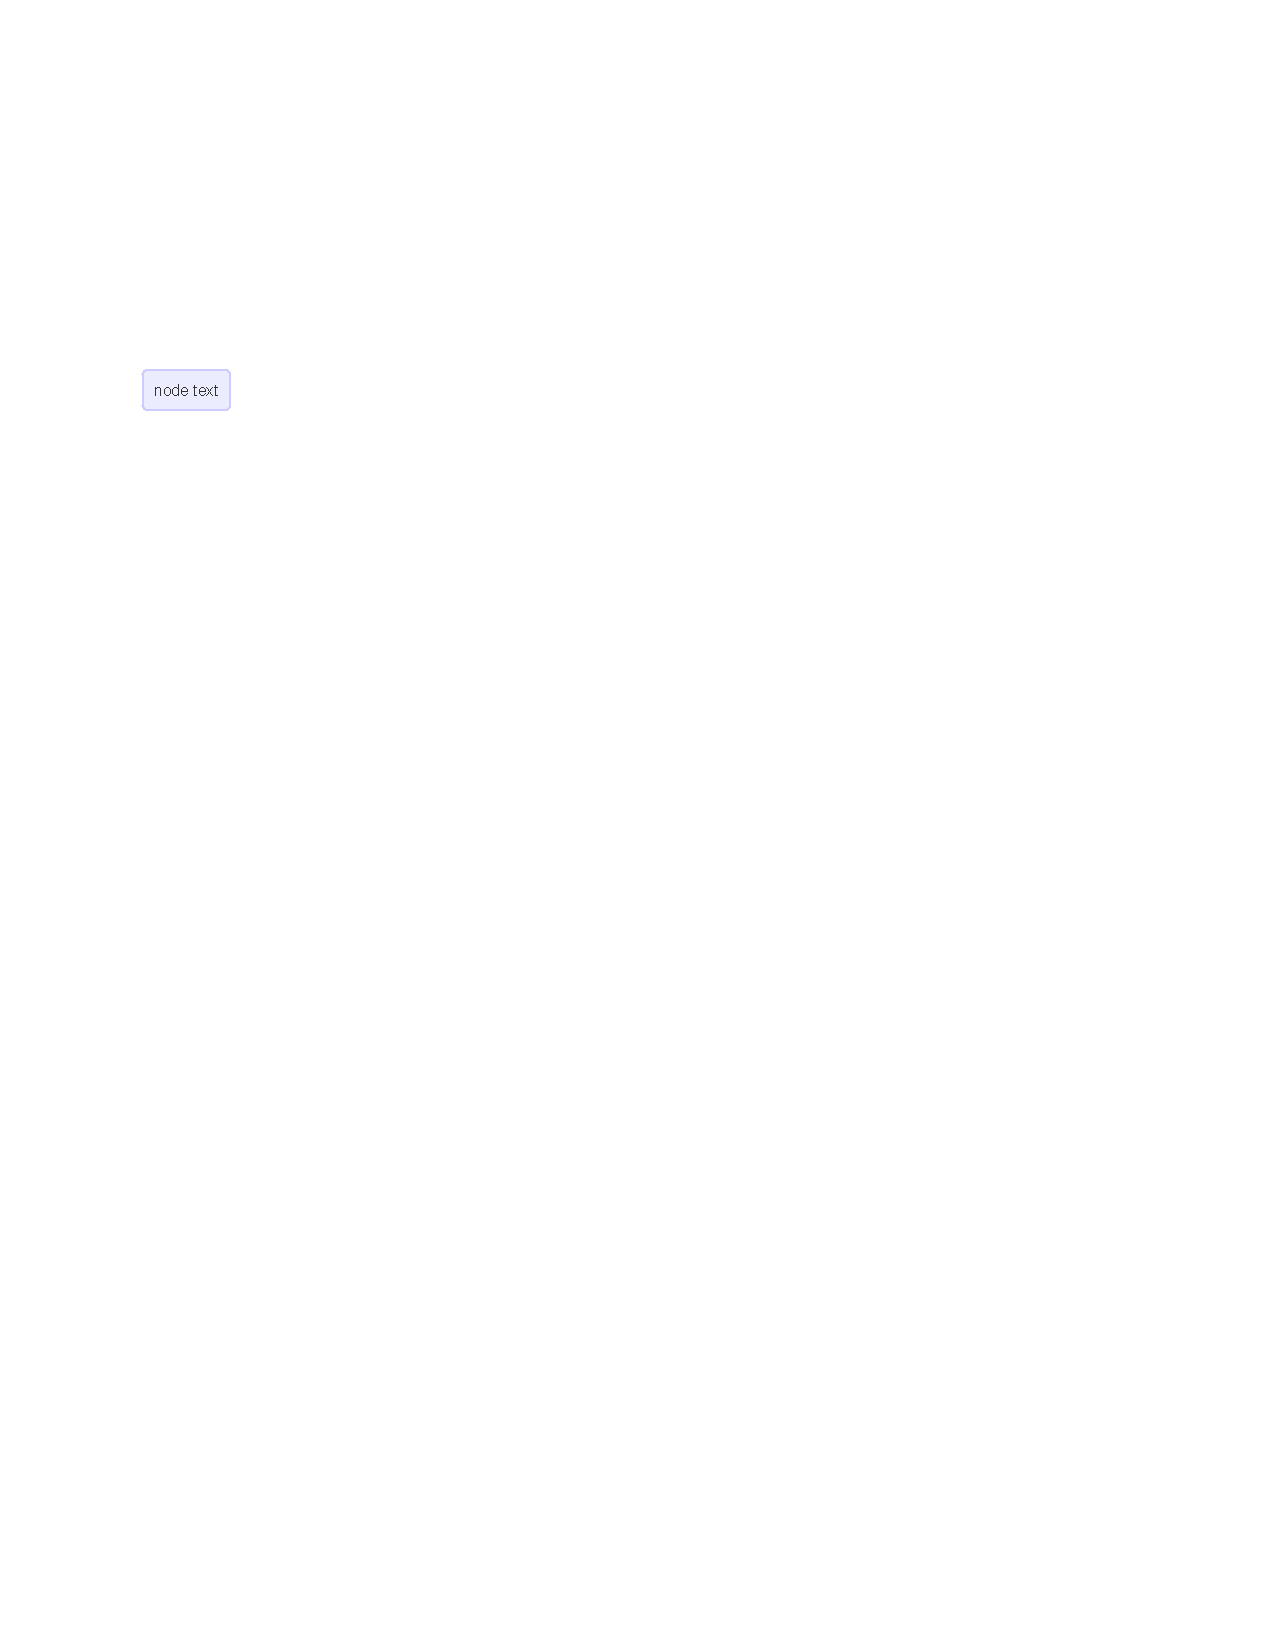
\includegraphics{./summary_files/figure-pdf/unnamed-chunk-4-2.pdf}


\includegraphics{./summary_files/figure-pdf/unnamed-chunk-4-3.pdf}

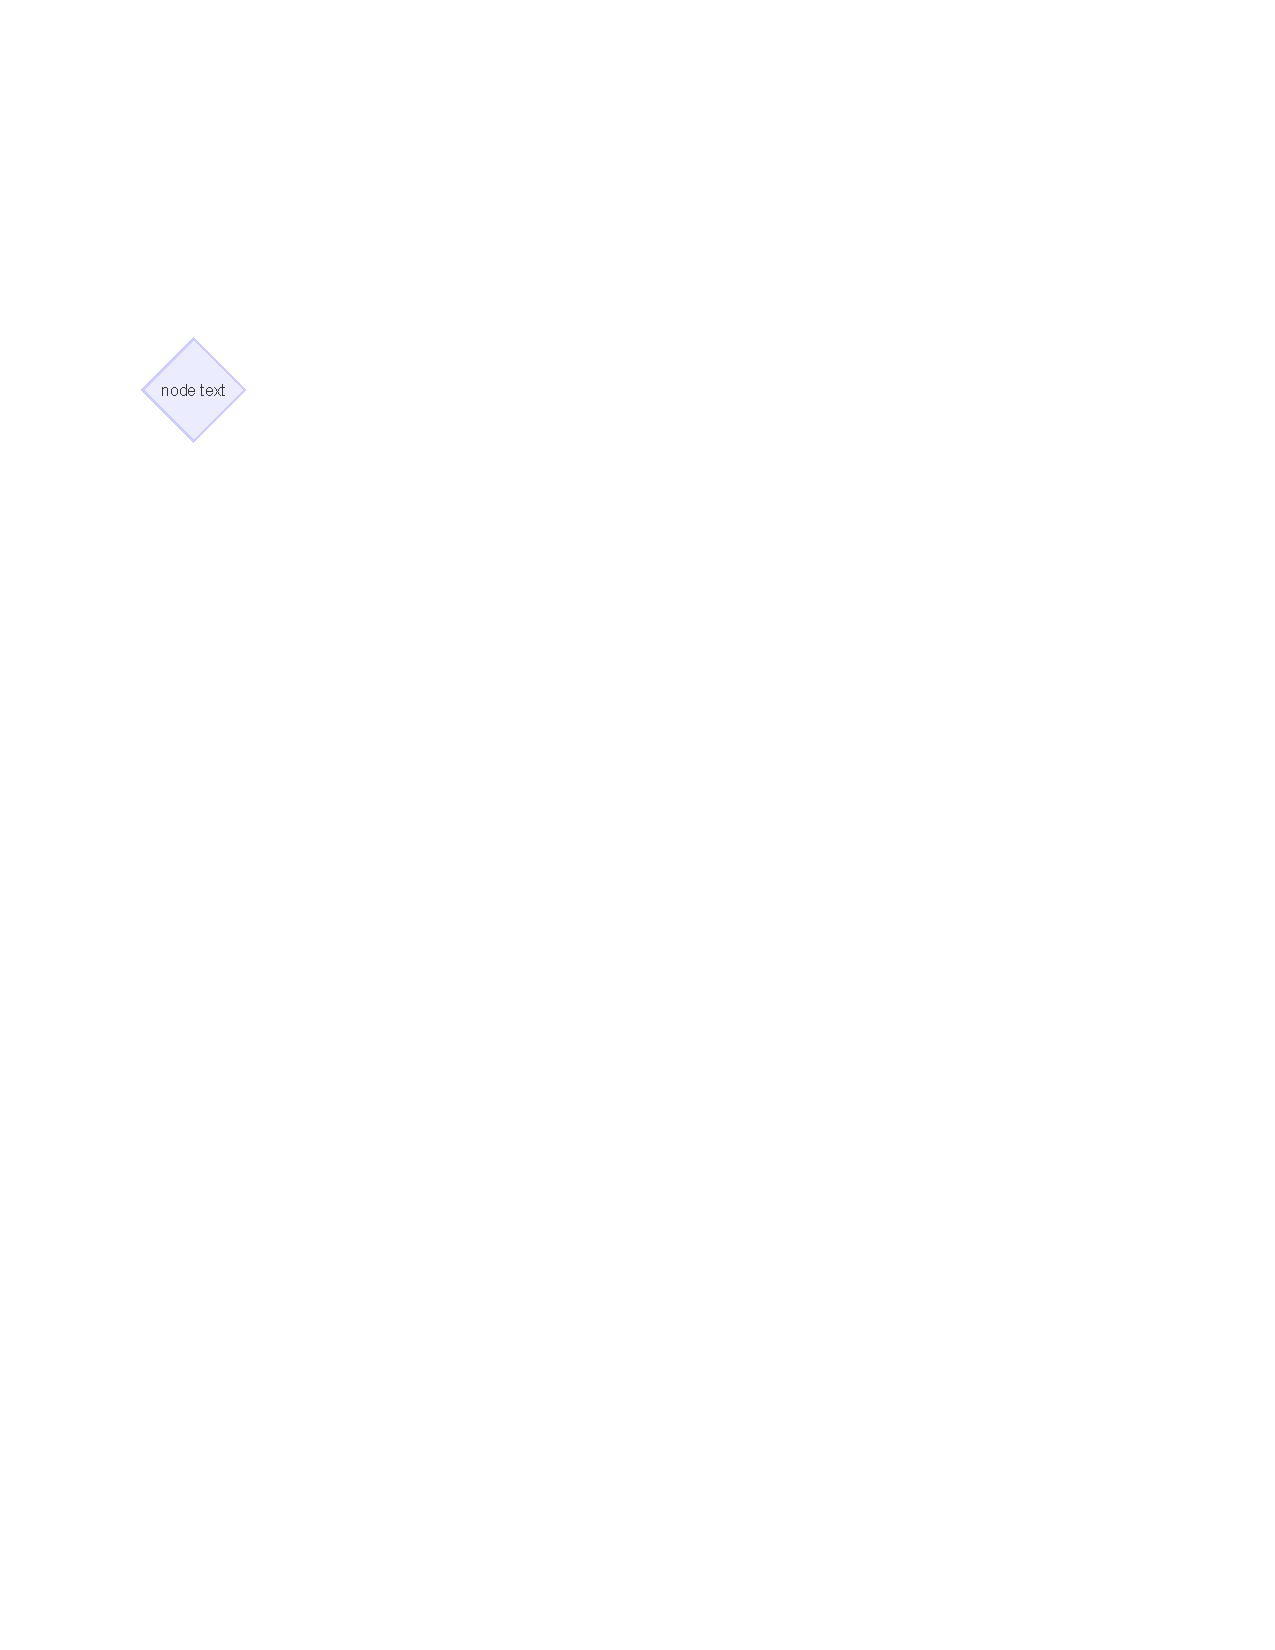
\includegraphics{./summary_files/figure-pdf/unnamed-chunk-4-4.pdf}

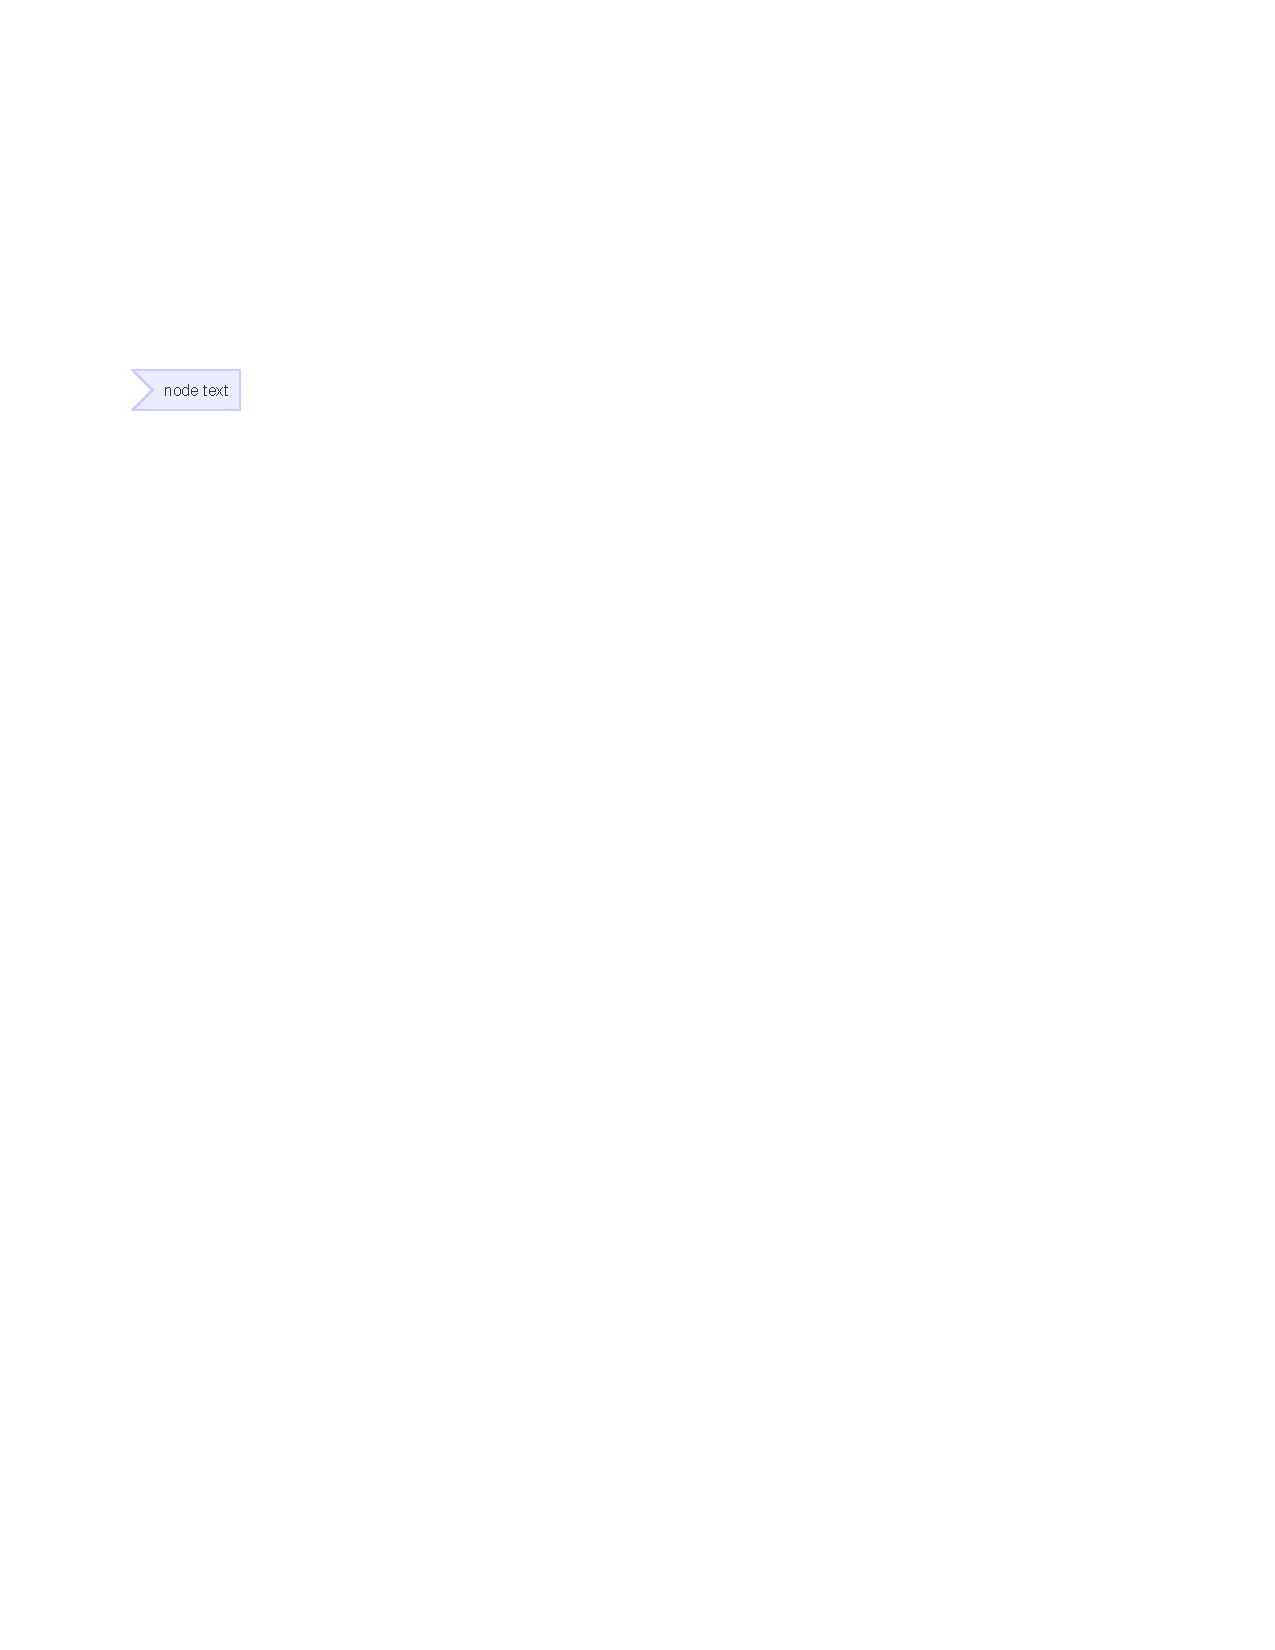
\includegraphics{./summary_files/figure-pdf/unnamed-chunk-4-5.pdf}

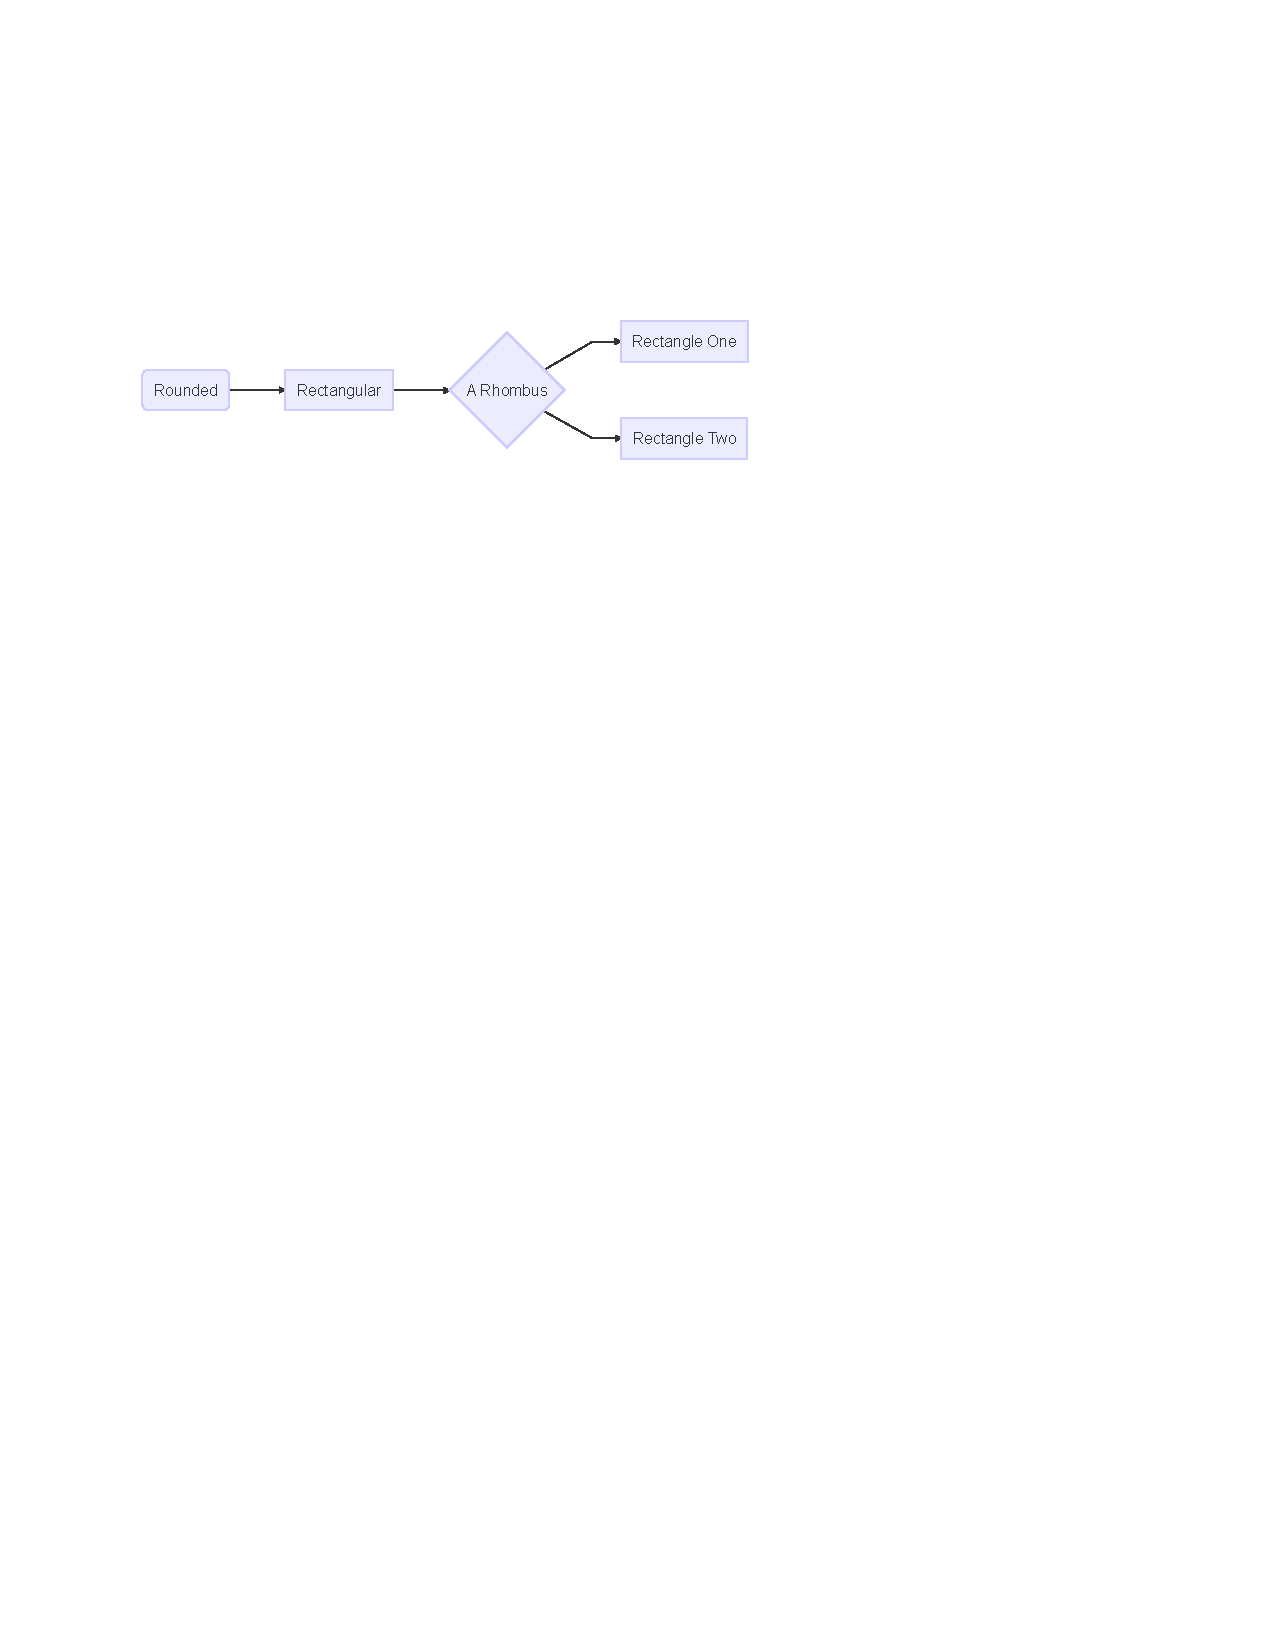
\includegraphics{./summary_files/figure-pdf/unnamed-chunk-4-6.pdf}

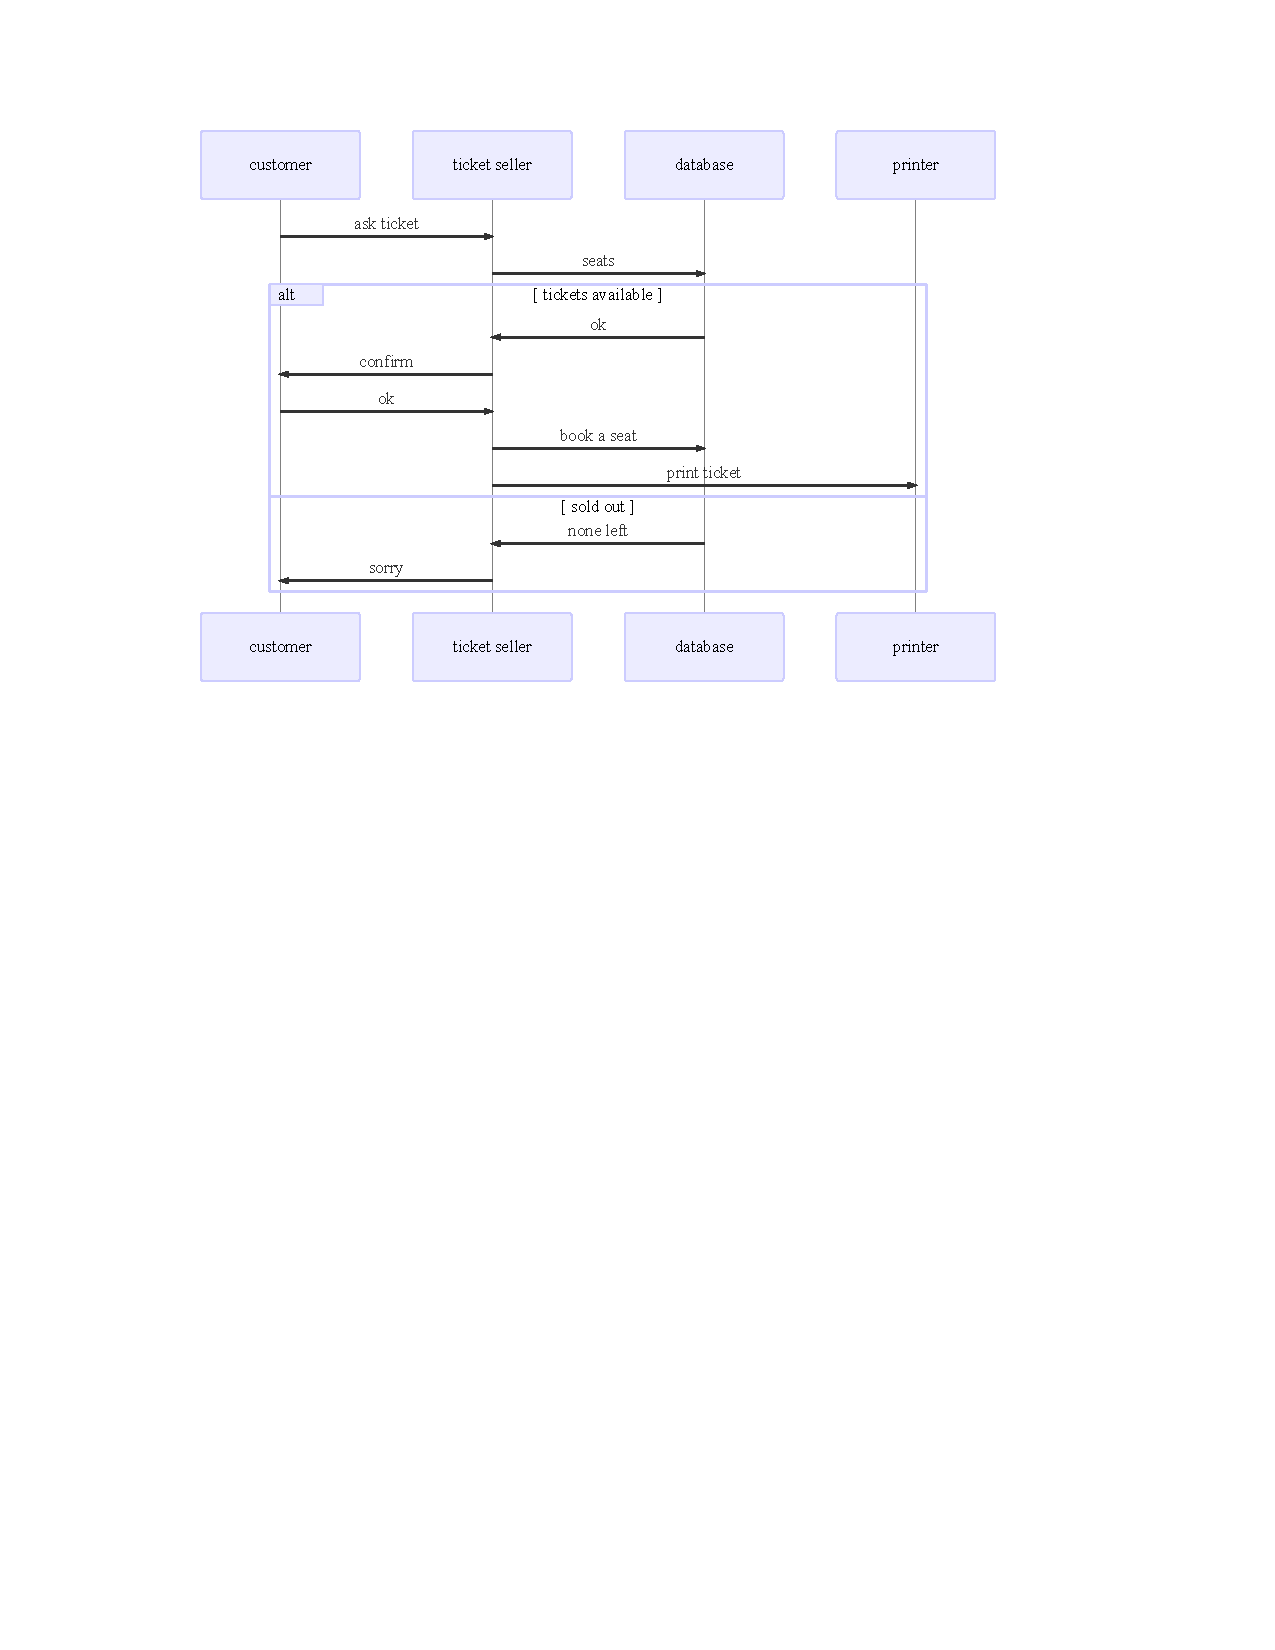
\includegraphics{./summary_files/figure-pdf/unnamed-chunk-5-1.pdf}

\bookmarksetup{startatroot}

\hypertarget{references}{%
\chapter*{References}\label{references}}
\addcontentsline{toc}{chapter}{References}

\markboth{References}{References}

\hypertarget{refs}{}
\begin{CSLReferences}{1}{0}
\leavevmode\vadjust pre{\hypertarget{ref-ecke2008babylonia}{}}%
Ecke, Peter. 2008. {``Die Kosten Der Mehrsprachigkeit.''}
\emph{Babylonia}, no. 2: 26--30.
\url{http://www.u.arizona.edu/~eckep/Ecke\%2008\%20Kosten\%20der\%20MS.pdf}.

\leavevmode\vadjust pre{\hypertarget{ref-kauschke2012kindlicher}{}}%
Kauschke, Christina. 2012. \emph{Kindlicher Spracherwerb Im Deutschen:
Verl{ä}ufe, Forschungsmethoden, Erkl{ä}rungsans{ä}tze}. Vol. 45. walter
de Gruyter.

\end{CSLReferences}


\backmatter

\printindex

\end{document}
